% Requires in the preamble:
% \usepackage{amsmath,amssymb}
% \usepackage{tikz,pgfplots}
% \pgfplotsset{compat=1.18}

\chapter{Power Series, Taylor Polynomials, and Taylor Series}
\label{chap:power-series-taylor}

The last chapter ended with a change in viewpoint.

A numerical series is an infinite sum of numbers:

\[
\sum_{n=1}^{\infty} a_n.
\]

Now the terms will depend on \(x\):

\[
a_0+a_1x+a_2x^2+a_3x^3+\cdots.
\]

Then the infinite sum is no longer only a number.  It can become a function.

This is a large step.  Polynomials are the friendliest functions in calculus.  We can add
them, multiply them, differentiate them, and integrate them term by term.  A power
series asks whether we can keep those polynomial habits when the polynomial has
infinitely many terms.

\[
\boxed{
\text{A power series is an infinite polynomial, but only where it converges.}
}
\]

That last phrase is the warning.  A power series may behave beautifully near its center
and fail completely farther away.

\section{Power series}
\label{sec:power-series}

The simplest infinite polynomial is

\[
1+x+x^2+x^3+\cdots.
\]

For a fixed value of \(x\), this becomes a numerical series.  The same formula can
converge for some inputs and diverge for others.

That is the first new question:

\[
\boxed{
\text{For which \(x\)-values does the infinite polynomial make sense?}
}
\]

\subsection{A polynomial with infinitely many terms}
\label{subsec:polynomial-with-infinitely-many-terms}

Start with

\[
1+x+x^2+x^3+\cdots.
\]

If \(x=\frac12\), then the series becomes

\[
1+\frac12+\frac14+\frac18+\cdots.
\]

This is a geometric series with ratio \(\frac12\), so it converges.

If \(x=2\), then the series becomes

\[
1+2+4+8+\cdots,
\]

which diverges.

If \(x=1\), then the series becomes

\[
1+1+1+1+\cdots,
\]

which diverges.

If \(x=-1\), then the series becomes

\[
1-1+1-1+\cdots,
\]

whose partial sums are

\[
1,\ 0,\ 1,\ 0,\ldots.
\]

Those partial sums do not approach one number, so the series diverges.

The same expression

\[
1+x+x^2+x^3+\cdots
\]

therefore behaves differently at different \(x\)-values.  It converges at
\(x=\frac12\), but diverges at \(x=2\), \(x=1\), and \(x=-1\).

A finite polynomial does not have this issue.  For example,

\[
1+x+x^2+x^3
\]

is defined for every real number \(x\).  There are only four terms to add.  An infinite
polynomial needs a convergence test at each input.

\begin{quote}
\textbf{Power series centered at \(0\).}
A \emph{power series centered at \(0\)} is a series of the form

\[
\boxed{
\sum_{n=0}^{\infty} c_n x^n
=
c_0+c_1x+c_2x^2+c_3x^3+\cdots.
}
\]

The constants \(c_0,c_1,c_2,\ldots\) are called the \emph{coefficients} of the power
series.
\end{quote}

The word ``power'' comes from the powers

\[
1,\ x,\ x^2,\ x^3,\ldots.
\]

For each fixed \(x\), the power series becomes the numerical series

\[
\sum_{n=0}^{\infty} c_n x^n.
\]

It may converge or diverge.  The set of all \(x\)-values where it converges is called
the \emph{interval of convergence}.

\paragraph{Example.}
Consider

\[
\sum_{n=0}^{\infty} x^n.
\]

This is the series

\[
1+x+x^2+x^3+\cdots.
\]

For a fixed \(x\), it is a geometric series with ratio \(x\).  Therefore it converges
when

\[
|x|<1,
\]

and diverges when

\[
|x|\ge 1.
\]

So its interval of convergence is

\[
\boxed{(-1,1).}
\]

Later we will use the geometric series to represent a familiar function.  For now, the
important lesson is simpler: a power series comes with a domain, and that domain
must be found.

\subsection{Center of a power series}
\label{subsec:center-of-power-series}

Power series do not have to be centered at \(0\).  They can be centered at any real
number \(a\).

For example,

\[
1+(x-3)+(x-3)^2+(x-3)^3+\cdots
\]

is built from powers of \(x-3\).  Its center is \(3\).  At \(x=3\), every term after the
first is \(0\), so the series becomes

\[
1+0+0+0+\cdots.
\]

The center is always included in the interval of convergence.

\begin{quote}
\textbf{Power series centered at \(a\).}
A \emph{power series centered at \(a\)} is a series of the form

\[
\boxed{
\sum_{n=0}^{\infty} c_n(x-a)^n
=
c_0+c_1(x-a)+c_2(x-a)^2+\cdots.
}
\]

The number \(a\) is called the \emph{center} of the power series.
\end{quote}

The expression \(x-a\) measures the signed distance from \(x\) to the center.  That is
why convergence will be controlled by

\[
|x-a|.
\]

Power series usually converge near their center and fail farther away.

\paragraph{Example.}
Find where the power series

\[
\sum_{n=0}^{\infty}\left(\frac{x-3}{2}\right)^n
\]

converges.

For a fixed \(x\), this is a geometric series with ratio

\[
r=\frac{x-3}{2}.
\]

It converges when

\[
|r|<1.
\]

Thus

\[
\left|\frac{x-3}{2}\right|<1.
\]

Multiply by \(2\):

\[
|x-3|<2.
\]

This means

\[
1<x<5.
\]

Now test the endpoints.

At \(x=1\),

\[
\frac{x-3}{2}=-1,
\]

so the series becomes

\[
1-1+1-1+\cdots,
\]

which diverges.

At \(x=5\),

\[
\frac{x-3}{2}=1,
\]

so the series becomes

\[
1+1+1+1+\cdots,
\]

which diverges.

Therefore the interval of convergence is

\[
\boxed{(1,5).}
\]

The interval is centered at \(3\), with distance \(2\) to each endpoint.

\subsection{Radius and interval of convergence}
\label{subsec:radius-interval-convergence}

The examples suggest a pattern.  A power series converges in a symmetric region
around its center.  The endpoints need separate attention.

\begin{figure}[h]
\centering
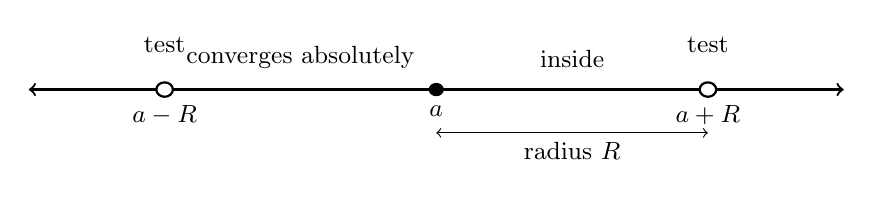
\begin{tikzpicture}[xscale=1.15, every node/.style={font=\small}]
  \draw[<->, thick] (-4.5,0) -- (4.5,0);

  \draw[very thick] (-3,0) -- (3,0);
  \draw[fill=white, thick] (-3,0) circle (2.6pt);
  \draw[fill=white, thick] (3,0) circle (2.6pt);
  \draw[fill=black] (0,0) circle (2.2pt);

  \node[below] at (-3,-0.08) {\(a-R\)};
  \node[below] at (0,-0.08) {\(a\)};
  \node[below] at (3,-0.08) {\(a+R\)};

  \node[above] at (-1.5,0.15) {converges absolutely};
  \node[above] at (1.5,0.15) {inside};
  \node[above] at (-3,0.35) {test};
  \node[above] at (3,0.35) {test};

  \draw[<->] (0,-0.55) -- (3,-0.55);
  \node[below] at (1.5,-0.55) {radius \(R\)};
\end{tikzpicture}
\caption{A power series has a center \(a\) and a radius of convergence \(R\).  Endpoint behavior is not decided by the radius alone.}
\label{fig:radius-of-convergence}
\end{figure}

\begin{quote}
\textbf{Radius of convergence.}
For a power series

\[
\sum_{n=0}^{\infty} c_n(x-a)^n,
\]

exactly one of the following happens.

\begin{enumerate}
\item The series converges only at its center \(x=a\).  Then the radius of convergence is
\[
R=0.
\]

\item The series converges for every real number \(x\).  Then the radius of convergence is
\[
R=\infty.
\]

\item There is a positive number \(R\) such that the series converges absolutely when
\[
|x-a|<R
\]
and diverges when
\[
|x-a|>R.
\]
The endpoints
\[
x=a-R
\qquad\text{and}\qquad
x=a+R
\]
must be tested separately.
\end{enumerate}
\end{quote}

The \emph{interval of convergence} is the full set of \(x\)-values where the series
converges.  It depends on the radius and on what happens at the endpoints.

\paragraph{Why the convergence set is an interval.}
Here is the main idea.

Suppose the power series

\[
\sum_{n=0}^{\infty} c_n(x-a)^n
\]

converges at some point \(x_1\neq a\).  Let

\[
r_1=|x_1-a|.
\]

Then the terms

\[
c_n(x_1-a)^n
\]

approach \(0\), so their absolute values are bounded.  That means there is some
number \(M\) such that

\[
|c_n(x_1-a)^n|\le M
\]

for all \(n\).

Now choose any \(x\) closer to the center than \(x_1\) is:

\[
|x-a|<|x_1-a|.
\]

Set

\[
q=\frac{|x-a|}{|x_1-a|}.
\]

Then

\[
0\le q<1.
\]

For each \(n\),

\[
|c_n(x-a)^n|
=
|c_n(x_1-a)^n|
\left(\frac{|x-a|}{|x_1-a|}\right)^n
\le
Mq^n.
\]

But

\[
\sum_{n=0}^{\infty} Mq^n
\]

is a convergent geometric series.  By comparison,

\[
\sum_{n=0}^{\infty} |c_n(x-a)^n|
\]

converges.  So the original power series converges absolutely at every point closer
to the center.

This explains the shape: once a power series converges at one point, it converges at
all points closer to the center.

The opposite statement follows by the same logic.  If the series diverges at some
point, it must diverge at every point farther from the center.  Otherwise convergence
farther out would force convergence closer in.

That is why the convergence set is an interval centered at \(a\), with possible choices
about the two endpoints.

\paragraph{Example: infinite radius.}
Find the radius of convergence of

\[
\sum_{n=0}^{\infty}\frac{x^n}{n!}.
\]

Use the Ratio Test.  Let

\[
a_n=\frac{x^n}{n!}.
\]

Then

\[
\left|\frac{a_{n+1}}{a_n}\right|
=
\left|\frac{x^{n+1}}{(n+1)!}\cdot \frac{n!}{x^n}\right|
=
\frac{|x|}{n+1}.
\]

As \(n\to\infty\),

\[
\frac{|x|}{n+1}\to0
\]

for every fixed real number \(x\).  Since the ratio limit is always less than \(1\), the
series converges for every \(x\).

Therefore

\[
\boxed{R=\infty}
\]

and the interval of convergence is

\[
\boxed{(-\infty,\infty).}
\]

This series will become one of the most important series in calculus.

\paragraph{Example: radius zero.}
Find the radius of convergence of

\[
\sum_{n=0}^{\infty} n!x^n.
\]

Again use the Ratio Test.  Let

\[
a_n=n!x^n.
\]

Then

\[
\left|\frac{a_{n+1}}{a_n}\right|
=
\left|\frac{(n+1)!x^{n+1}}{n!x^n}\right|
=
(n+1)|x|.
\]

If \(x\neq0\), then

\[
(n+1)|x|\to\infty.
\]

So the series diverges for every \(x\neq0\).  At the center \(x=0\), the series becomes

\[
1+0+0+0+\cdots,
\]

which converges.

Therefore the series converges only at \(x=0\), and

\[
\boxed{R=0.}
\]

Not every power series gives a useful function on an interval.  Some collapse to a
single point.

\subsection{Endpoint testing}
\label{subsec:endpoint-testing-power-series}

The radius tells us what happens inside and outside.  It does not tell us what happens
at the endpoints.

The reason is simple: the Ratio Test often gives the limiting value \(1\) at the endpoints,
and the Ratio Test is silent when the limit is \(1\).

\paragraph{Example: one endpoint included.}
Find the interval of convergence of

\[
\sum_{n=1}^{\infty}\frac{x^n}{n}.
\]

For \(x\neq0\), use the Ratio Test on the absolute values:

\[
\left|
\frac{x^{n+1}}{n+1}\cdot\frac{n}{x^n}
\right|
=
|x|\frac{n}{n+1}.
\]

As \(n\to\infty\),

\[
|x|\frac{n}{n+1}\to |x|.
\]

So the series converges absolutely when

\[
|x|<1
\]

and diverges when

\[
|x|>1.
\]

The radius is

\[
R=1.
\]

Now test the endpoints.

At \(x=1\), the series becomes

\[
\sum_{n=1}^{\infty}\frac1n,
\]

the harmonic series.  It diverges.

At \(x=-1\), the series becomes

\[
\sum_{n=1}^{\infty}\frac{(-1)^n}{n}.
\]

This is an alternating harmonic series.  It converges by the Alternating Series Test.

Therefore the interval of convergence is

\[
\boxed{[-1,1).}
\]

One endpoint is included, and the other is not.

\paragraph{Example: both endpoints included.}
Find the interval of convergence of

\[
\sum_{n=1}^{\infty}\frac{(x-2)^n}{n^2}.
\]

Use the Ratio Test on absolute values:

\[
\left|
\frac{(x-2)^{n+1}}{(n+1)^2}\cdot \frac{n^2}{(x-2)^n}
\right|
=
|x-2|\frac{n^2}{(n+1)^2}.
\]

As \(n\to\infty\),

\[
|x-2|\frac{n^2}{(n+1)^2}\to |x-2|.
\]

Thus the series converges absolutely when

\[
|x-2|<1,
\]

or

\[
1<x<3.
\]

The radius is \(1\), centered at \(2\).

Now test endpoints.

At \(x=1\), the series becomes

\[
\sum_{n=1}^{\infty}\frac{(-1)^n}{n^2}.
\]

This converges absolutely because

\[
\sum_{n=1}^{\infty}\frac1{n^2}
\]

converges.

At \(x=3\), the series becomes

\[
\sum_{n=1}^{\infty}\frac1{n^2},
\]

which also converges.

Therefore the interval of convergence is

\[
\boxed{[1,3].}
\]

\begin{quote}
\textbf{Endpoint checklist.}

After finding the radius \(R\), do not stop at

\[
|x-a|<R.
\]

Test

\[
x=a-R
\qquad\text{and}\qquad
x=a+R
\]

as two ordinary numerical series.  Use the tests from Chapter \ref{chap:sequences-infinite-series}:
geometric, \(p\)-series, comparison, alternating, ratio, root, or term test.
\end{quote}

The next section shows why power series are worth this work.  Inside their interval of
convergence, they can be handled almost like polynomials.

\section{Working with power series}
\label{sec:working-with-power-series}

A power series first asks where it converges.  Once we are safely inside that interval,
a second question begins:

\[
\boxed{
\text{Can we calculate with it as if it were a polynomial?}
}
\]

The answer is mostly yes, but the words ``safely inside'' matter.  Inside the radius of
convergence, power series are unusually well behaved.  At endpoints, every operation
must be checked again.

\subsection{Algebra of power series}
\label{subsec:algebra-of-power-series}

Finite polynomials can be added term by term:

\[
(1+2x+3x^2)+(4-x+5x^2)=5+x+8x^2.
\]

Power series can also be added term by term where both series converge.

Suppose

\[
F(x)=\sum_{n=0}^{\infty} a_n(x-c)^n
\]

and

\[
G(x)=\sum_{n=0}^{\infty} b_n(x-c)^n
\]

are power series with the same center \(c\).  Wherever both series converge, their
sum is

\[
F(x)+G(x)
=
\sum_{n=0}^{\infty}\bigl(a_n+b_n\bigr)(x-c)^n.
\]

Similarly,

\[
F(x)-G(x)
=
\sum_{n=0}^{\infty}\bigl(a_n-b_n\bigr)(x-c)^n.
\]

\begin{quote}
\textbf{Adding power series.}
If two power series have the same center, then inside any interval where both
converge absolutely,

\[
\boxed{
\sum_{n=0}^{\infty} a_n(x-c)^n
+
\sum_{n=0}^{\infty} b_n(x-c)^n
=
\sum_{n=0}^{\infty}(a_n+b_n)(x-c)^n.
}
\]

The same rule works for subtraction.
\end{quote}

At minimum, this is safe inside the smaller of the two radii of convergence.  Sometimes
the resulting series may converge farther because of cancellation, but the common
interior is the guaranteed region.

\paragraph{Example.}
Let

\[
F(x)=\sum_{n=1}^{\infty}\frac{x^n}{n}
\]

and

\[
G(x)=\sum_{n=1}^{\infty}\frac{x^n}{n^2}.
\]

Both have radius \(1\).  For \(|x|<1\),

\[
F(x)+G(x)
=
\sum_{n=1}^{\infty}\left(\frac1n+\frac1{n^2}\right)x^n.
\]

This is just coefficient-by-coefficient addition.

\paragraph{Multiplying by a power of \(x\).}
If

\[
F(x)=\sum_{n=0}^{\infty} c_nx^n,
\]

then

\[
x^2F(x)
=
\sum_{n=0}^{\infty} c_nx^{n+2}.
\]

This shifts the powers upward by \(2\).  For example,

\[
x^2(1+x+x^2+x^3+\cdots)
=
x^2+x^3+x^4+x^5+\cdots.
\]

This kind of shift is one of the most common algebra moves with power series.

\paragraph{Multiplying two power series.}
Multiplication is a little more delicate.  Every term in one series can multiply every
term in the other.  The coefficient of a given power collects all products whose powers
add to that value.

If

\[
F(x)=\sum_{n=0}^{\infty} a_nx^n
\]

and

\[
G(x)=\sum_{n=0}^{\infty} b_nx^n,
\]

then the product has the form

\[
F(x)G(x)
=
\sum_{n=0}^{\infty} d_nx^n,
\]

where

\[
\boxed{
d_n=a_0b_n+a_1b_{n-1}+a_2b_{n-2}+\cdots+a_nb_0.
}
\]

Equivalently,

\[
\boxed{
d_n=\sum_{k=0}^{n} a_k b_{n-k}.
}
\]

This is called the \emph{Cauchy product}.

\paragraph{Example.}
Multiply

\[
(1+x+x^2+x^3+\cdots)
\]

by itself.

The coefficient of \(x^0\) is

\[
1.
\]

The coefficient of \(x^1\) is

\[
1+1=2,
\]

because

\[
x^1=x\cdot1+1\cdot x.
\]

The coefficient of \(x^2\) is

\[
1+1+1=3,
\]

because

\[
x^2=x^2\cdot1+x\cdot x+1\cdot x^2.
\]

In general, the coefficient of \(x^n\) is \(n+1\).  Therefore, for \(|x|<1\),

\[
(1+x+x^2+\cdots)^2
=
\sum_{n=0}^{\infty}(n+1)x^n.
\]

We have not yet identified the left side as a familiar function.  We are only using the
algebra of the infinite polynomial where the series converges absolutely.

\subsection{Differentiating power series}
\label{subsec:differentiating-power-series}

A finite polynomial can be differentiated term by term:

\[
\frac{d}{dx}\left(c_0+c_1x+c_2x^2+c_3x^3\right)
=
c_1+2c_2x+3c_3x^2.
\]

A power series can also be differentiated term by term inside its radius of convergence.

\begin{quote}
\textbf{Term-by-term differentiation of a power series.}
Suppose

\[
F(x)=\sum_{n=0}^{\infty} c_n(x-a)^n
\]

has radius of convergence \(R>0\).  Then \(F\) is differentiable for

\[
|x-a|<R,
\]

and

\[
\boxed{
F'(x)=\sum_{n=1}^{\infty} n c_n(x-a)^{n-1}
}
\]

for every \(x\) satisfying \(|x-a|<R\).

The differentiated series has the same radius of convergence \(R\).  Endpoint behavior
must be checked separately.
\end{quote}

This theorem is one of the reasons power series are so useful.  An infinite polynomial
can still be differentiated like a polynomial, as long as we stay inside its radius.

\paragraph{Example.}
Let

\[
F(x)=\sum_{n=0}^{\infty} x^n
=
1+x+x^2+x^3+\cdots.
\]

This series has radius \(1\).  For \(|x|<1\),

\[
F'(x)
=
\sum_{n=1}^{\infty} n x^{n-1}.
\]

So

\[
F'(x)=1+2x+3x^2+4x^3+\cdots,
\qquad |x|<1.
\]

The differentiated series also has radius \(1\).

\paragraph{Example.}
Let

\[
G(x)=\sum_{n=1}^{\infty}\frac{x^n}{n}.
\]

From the previous section, \(G\) has radius \(1\).  For \(|x|<1\),

\[
G'(x)
=
\sum_{n=1}^{\infty}\frac{n x^{n-1}}{n}
=
\sum_{n=1}^{\infty}x^{n-1}.
\]

Thus

\[
\boxed{
G'(x)=1+x+x^2+x^3+\cdots,
\qquad |x|<1.
}
\]

Notice what happened at the endpoints.

The original series

\[
\sum_{n=1}^{\infty}\frac{x^n}{n}
\]

converges at \(x=-1\) and diverges at \(x=1\).  The derivative series

\[
\sum_{n=1}^{\infty}x^{n-1}
\]

diverges at both \(x=-1\) and \(x=1\).

The radius is the same, but endpoint behavior changed.

\begin{quote}
\textbf{Endpoint warning.}
Term-by-term differentiation is guaranteed only for

\[
|x-a|<R.
\]

Even if the original series converges at an endpoint, the differentiated series may
diverge there.
\end{quote}

\subsection{Integrating power series}
\label{subsec:integrating-power-series}

Power series can also be integrated term by term inside their radius of convergence.

\begin{quote}
\textbf{Term-by-term integration of a power series.}
Suppose

\[
F(x)=\sum_{n=0}^{\infty} c_n(x-a)^n
\]

has radius of convergence \(R>0\).  Then for \(|x-a|<R\),

\[
\boxed{
\int F(x)\,dx
=
C+\sum_{n=0}^{\infty} c_n\frac{(x-a)^{n+1}}{n+1}.
}
\]

Equivalently,

\[
\boxed{
\int_a^x F(t)\,dt
=
\sum_{n=0}^{\infty} c_n\frac{(x-a)^{n+1}}{n+1},
\qquad |x-a|<R.
}
\]

The integrated series has the same radius of convergence \(R\).  Endpoint behavior
must be checked separately.
\end{quote}

The definite-integral version fits the accumulation story.  Each term

\[
c_n(t-a)^n\,dt
\]

is accumulated from \(a\) to \(x\), giving

\[
c_n\frac{(x-a)^{n+1}}{n+1}.
\]

The small step \(dt\) carries the direction of accumulation, just as it did in the
Fundamental Theorem.

\paragraph{Example.}
Integrate

\[
1+x+x^2+x^3+\cdots
\]

from \(0\) to \(x\).  For \(|x|<1\),

\[
\int_0^x (1+t+t^2+t^3+\cdots)\,dt
=
\int_0^x 1\,dt+\int_0^x t\,dt+\int_0^x t^2\,dt+\cdots.
\]

Therefore

\[
\boxed{
\int_0^x (1+t+t^2+t^3+\cdots)\,dt
=
x+\frac{x^2}{2}+\frac{x^3}{3}+\frac{x^4}{4}+\cdots,
\qquad |x|<1.
}
\]

The power series on the right still has radius \(1\), but its endpoint behavior is different
from the original geometric series.  At \(x=-1\), it becomes an alternating harmonic-type
series and converges.  At \(x=1\), it becomes the harmonic series and diverges.

So the interval of convergence for the integrated series is

\[
[-1,1).
\]

The theorem guaranteed the interval \((-1,1)\).  Endpoint testing gave the extra
information.

\paragraph{Example centered away from zero.}
Let

\[
F(x)=\sum_{n=0}^{\infty}\frac{(x-1)^n}{2^n}.
\]

This is a geometric series in

\[
\frac{x-1}{2},
\]

so it has radius \(2\), centered at \(1\).  For

\[
|x-1|<2,
\]

we may integrate term by term:

\[
\int_1^x F(t)\,dt
=
\sum_{n=0}^{\infty}
\frac{(x-1)^{n+1}}{(n+1)2^n}.
\]

So

\[
\boxed{
\int_1^x \left(\sum_{n=0}^{\infty}\frac{(t-1)^n}{2^n}\right)dt
=
\sum_{n=0}^{\infty}
\frac{(x-1)^{n+1}}{(n+1)2^n},
\qquad |x-1|<2.
}
\]

The center \(1\) remains visible.  The powers are still powers of \(x-1\).

\subsection{Why power series behave better than arbitrary series}
\label{subsec:why-power-series-behave-better}

Term-by-term differentiation and integration are not gifts we receive for every infinite
sum of functions.  They are special properties of power series inside their radius of
convergence.

The reason is that power series have a geometric safety margin.

Suppose

\[
\sum_{n=0}^{\infty} c_n(x-a)^n
\]

has radius \(R\).  Choose a smaller distance \(r\) with

\[
0<r<R.
\]

Then every \(x\) in the closed interval

\[
a-r\le x\le a+r
\]

lies safely inside the radius.

\begin{figure}[h]
\centering
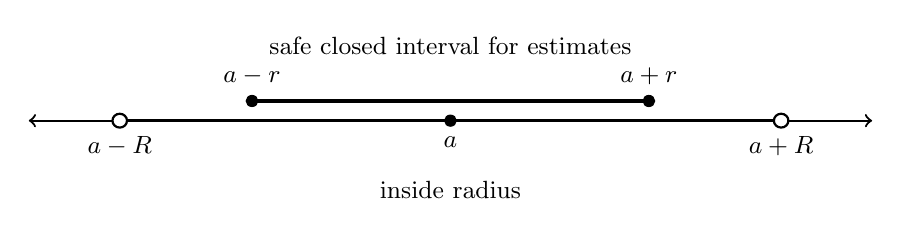
\begin{tikzpicture}[xscale=1.05, every node/.style={font=\small}]
  \draw[<->, thick] (-5.1,0) -- (5.1,0);

  % Outer radius interval
  \draw[very thick] (-4,0) -- (4,0);
  \draw[fill=white, thick] (-4,0) circle (2.5pt);
  \draw[fill=white, thick] (4,0) circle (2.5pt);

  % Inner safe interval
  \draw[very thick] (-2.4,0.25) -- (2.4,0.25);
  \draw[fill=black] (-2.4,0.25) circle (2pt);
  \draw[fill=black] (2.4,0.25) circle (2pt);
  \draw[fill=black] (0,0) circle (2pt);

  \node[below] at (-4,-0.08) {\(a-R\)};
  \node[below] at (0,-0.08) {\(a\)};
  \node[below] at (4,-0.08) {\(a+R\)};

  \node[above] at (-2.4,0.33) {\(a-r\)};
  \node[above] at (2.4,0.33) {\(a+r\)};

  \node[below] at (0,-0.65) {inside radius};
  \node[above] at (0,0.72) {safe closed interval for estimates};
\end{tikzpicture}
\caption{Inside a smaller interval \([a-r,a+r]\), a power series is controlled uniformly by geometric bounds.}
\label{fig:safe-interval-inside-radius}
\end{figure}

Because \(r<R\), we can choose a number \(\rho\) such that

\[
r<\rho<R.
\]

The series converges absolutely at distance \(\rho\) from the center:

\[
\sum_{n=0}^{\infty}|c_n|\rho^n
\]

converges.

For every \(x\) with \(|x-a|\le r\),

\[
|c_n(x-a)^n|
\le
|c_n|r^n.
\]

The numerical series

\[
\sum_{n=0}^{\infty}|c_n|r^n
\]

converges by comparison with the convergent series at distance \(\rho\).  So the power
series is controlled on the whole smaller interval, not just point by point.

That uniform control is what lets us safely pass limits through sums, derivatives, and
integrals.  A later optional section will give this idea a name: uniform convergence.

For now, the practical rule is enough.

\begin{quote}
\textbf{Safe operations inside the radius.}

If

\[
F(x)=\sum_{n=0}^{\infty} c_n(x-a)^n
\]

has radius \(R>0\), then for

\[
|x-a|<R
\]

we may:

\begin{enumerate}
\item add and subtract power series term by term, within a common radius;

\item multiply power series using coefficient collection;

\item differentiate term by term;

\item integrate term by term.
\end{enumerate}

At endpoints, test again.
\end{quote}

\begin{center}
\begin{tabular}{c|c|c}
\textbf{operation} & \textbf{inside the radius} & \textbf{at endpoints} \\ \hline
addition/subtraction & safe in common interior & test separately \\
multiplication & safe in common interior & test separately \\
differentiation & safe term by term & may fail \\
integration & safe term by term & may improve or fail
\end{tabular}
\end{center}

This is why power series are more than a new kind of series.  They are a new kind of
function-building machine.

The next step is to feed familiar functions into that machine.  The geometric series will
be the seed.  From it, we will build series for logarithms, inverse tangents, and soon
the functions that explain the mysterious formula

\[
e^{i\theta}=\cos\theta+i\sin\theta.
\]

\section{Representing functions by power series}
\label{sec:representing-functions-power-series}

The last section gave us permission to work with power series inside their radius of
convergence.  We can add, multiply, differentiate, and integrate them term by term.

Now we use that permission in the opposite direction.

Instead of starting with a power series and asking where it converges, we start with a
function and ask:

\[
\boxed{
\text{Can this function be written as an infinite polynomial?}
}
\]

The first seed is the geometric series.  From that one seed, differentiation,
integration, and substitution will grow new series.

\subsection{Geometric series as the seed}
\label{subsec:geometric-series-seed}

Start with the finite sum

\[
S_N(x)=1+x+x^2+\cdots+x^N.
\]

Multiply by \(1-x\):

\[
(1-x)S_N(x)
=
(1+x+x^2+\cdots+x^N)
-
(x+x^2+x^3+\cdots+x^{N+1}).
\]

Everything cancels except the first and last terms:

\[
(1-x)S_N(x)=1-x^{N+1}.
\]

So, if \(x\neq1\),

\[
S_N(x)=\frac{1-x^{N+1}}{1-x}.
\]

Now let \(N\to\infty\).  If

\[
|x|<1,
\]

then

\[
x^{N+1}\to0.
\]

Therefore

\[
S_N(x)\to \frac1{1-x}.
\]

Thus

\[
\boxed{
\frac1{1-x}=1+x+x^2+x^3+\cdots,
\qquad |x|<1.
}
\]

This is our first power series representation of a function.

\begin{figure}[h]
\centering
\begin{tikzpicture}
\begin{axis}[
    width=0.82\textwidth,
    height=0.50\textwidth,
    xmin=-0.85, xmax=0.85,
    ymin=0, ymax=5.8,
    axis lines=left,
    xlabel={\(x\)},
    ylabel={\(y\)},
    xtick={-0.8,-0.4,0,0.4,0.8},
    ytick={1,2,3,4,5},
    grid=both,
    grid style={line width=.1pt, draw=gray!25},
    legend style={draw=none, at={(0.03,0.97)}, anchor=north west}
]
\addplot[very thick, domain=-0.84:0.84, samples=200] {1/(1-x)};
\addlegendentry{\(\dfrac1{1-x}\)}

\addplot[thick, dashed, domain=-0.84:0.84, samples=200] {1+x};
\addlegendentry{\(1+x\)}

\addplot[thick, dotted, domain=-0.84:0.84, samples=200] {1+x+x^2+x^3};
\addlegendentry{\(1+x+x^2+x^3\)}

\addplot[thick, dashdotted, domain=-0.84:0.84, samples=200] {1+x+x^2+x^3+x^4+x^5+x^6+x^7};
\addlegendentry{\(S_7(x)\)}
\end{axis}
\end{tikzpicture}
\caption{Partial sums of the geometric series approach \(\frac1{1-x}\) on \((-1,1)\).}
\label{fig:geometric-partial-sums-function}
\end{figure}

The equality

\[
\frac1{1-x}=1+x+x^2+x^3+\cdots
\]

is not true for every \(x\).  At \(x=2\), the right side is

\[
1+2+4+8+\cdots,
\]

which diverges.  At \(x=-1\), the right side is

\[
1-1+1-1+\cdots,
\]

which also diverges.

So the formula always carries its home with it:

\[
\boxed{|x|<1.}
\]

A power series representation is not only an identity.  It is an identity together with
an interval where the identity is valid.

\subsection{\texorpdfstring{Series for \(\frac1{1-x}\)}{Series for 1/(1-x)}}
\label{subsec:series-for-one-over-one-minus-x}

The geometric series is a machine.  Once we know

\[
\frac1{1-x}=\sum_{n=0}^{\infty}x^n,
\qquad |x|<1,
\]

we can replace \(x\) by other expressions, as long as the new expression has absolute
value less than \(1\).

\paragraph{Example: replacing \(x\) by \(-x\).}
Since

\[
\frac1{1-u}=1+u+u^2+u^3+\cdots,
\qquad |u|<1,
\]

put

\[
u=-x.
\]

Then

\[
\frac1{1-(-x)}
=
1+(-x)+(-x)^2+(-x)^3+\cdots.
\]

So

\[
\boxed{
\frac1{1+x}
=
1-x+x^2-x^3+\cdots,
\qquad |x|<1.
}
\]

This will become the seed for the logarithm.

\paragraph{Example: replacing \(x\) by \(x^2\).}
Put

\[
u=x^2.
\]

Then

\[
\frac1{1-x^2}
=
1+x^2+x^4+x^6+\cdots.
\]

The condition is

\[
|x^2|<1,
\]

which is the same as

\[
|x|<1.
\]

Thus

\[
\boxed{
\frac1{1-x^2}
=
1+x^2+x^4+x^6+\cdots,
\qquad |x|<1.
}
\]

\paragraph{Example: a different radius.}
Find a power series for

\[
\frac1{2-x}
\]

centered at \(0\).

Rewrite the function so that the geometric form appears:

\[
\frac1{2-x}
=
\frac12\cdot \frac1{1-\frac{x}{2}}.
\]

Now use the geometric series with

\[
u=\frac{x}{2}.
\]

Then

\[
\frac1{1-\frac{x}{2}}
=
\sum_{n=0}^{\infty}\left(\frac{x}{2}\right)^n
\]

when

\[
\left|\frac{x}{2}\right|<1.
\]

So

\[
\boxed{
\frac1{2-x}
=
\sum_{n=0}^{\infty}\frac{x^n}{2^{n+1}},
\qquad |x|<2.
}
\]

The radius is \(2\), not \(1\), because the actual ratio is \(x/2\).

\paragraph{Example: a series centered at \(2\).}
Find a power series for

\[
\frac1x
\]

centered at \(2\).

Write \(x\) as

\[
x=2+(x-2).
\]

Then

\[
\frac1x
=
\frac1{2+(x-2)}
=
\frac12\cdot \frac1{1+\frac{x-2}{2}}.
\]

Use the series

\[
\frac1{1+u}=1-u+u^2-u^3+\cdots,
\qquad |u|<1,
\]

with

\[
u=\frac{x-2}{2}.
\]

Thus

\[
\boxed{
\frac1x
=
\frac12
-\frac{x-2}{4}
+\frac{(x-2)^2}{8}
-\frac{(x-2)^3}{16}
+\cdots
}
\]

or, more compactly,

\[
\boxed{
\frac1x
=
\sum_{n=0}^{\infty}
\frac{(-1)^n(x-2)^n}{2^{n+1}},
\qquad |x-2|<2.
}
\]

The center is \(2\).  The series converges when \(x\) is within distance \(2\) of that
center:

\[
0<x<4.
\]

This makes sense.  The function \(1/x\) has trouble at \(x=0\), and that point is exactly
distance \(2\) from the center \(2\).

\paragraph{Differentiating the geometric series.}
Inside \(|x|<1\),

\[
\frac1{1-x}=1+x+x^2+x^3+\cdots.
\]

Differentiate both sides:

\[
\frac{d}{dx}\left(\frac1{1-x}\right)
=
\frac{d}{dx}\left(1+x+x^2+x^3+\cdots\right).
\]

The left side is

\[
\frac1{(1-x)^2}.
\]

The right side is

\[
1+2x+3x^2+4x^3+\cdots.
\]

Therefore

\[
\boxed{
\frac1{(1-x)^2}
=
1+2x+3x^2+4x^3+\cdots,
\qquad |x|<1.
}
\]

This is the same product series we saw earlier:

\[
(1+x+x^2+\cdots)^2
=
1+2x+3x^2+4x^3+\cdots.
\]

The algebra and the calculus agree.

\begin{quote}
\textbf{A useful workflow.}

To represent a function by a power series:

\begin{enumerate}
\item Start from a known series, usually the geometric series.

\item Rewrite the function until the known pattern appears.

\item Substitute carefully.

\item State the convergence condition.

\item If you differentiate or integrate, keep the same radius but test endpoints again.
\end{enumerate}
\end{quote}

The endpoint warning is not decoration.  The next examples show why.

\subsection{\texorpdfstring{Series for \(\ln(1+x)\)}{Series for ln(1+x)}}
\label{subsec:series-for-log-one-plus-x}

The logarithm is connected to

\[
\frac1{1+x}
\]

because

\[
\frac{d}{dx}\ln(1+x)=\frac1{1+x}.
\]

We already found

\[
\frac1{1+x}
=
1-x+x^2-x^3+\cdots,
\qquad |x|<1.
\]

Integrate both sides from \(0\) to \(x\).  On the left,

\[
\int_0^x \frac1{1+t}\,dt
=
\ln(1+x)-\ln(1)
=
\ln(1+x).
\]

On the right,

\[
\int_0^x (1-t+t^2-t^3+\cdots)\,dt
=
x-\frac{x^2}{2}+\frac{x^3}{3}-\frac{x^4}{4}+\cdots.
\]

Therefore

\[
\boxed{
\ln(1+x)
=
x-\frac{x^2}{2}+\frac{x^3}{3}-\frac{x^4}{4}+\cdots,
\qquad -1<x<1.
}
\]

The theorem on integrating power series gives the equality inside the radius.  The
endpoints must be tested separately.

At \(x=1\), the series becomes

\[
1-\frac12+\frac13-\frac14+\frac15-\cdots.
\]

This converges by the Alternating Series Test.

At \(x=-1\), the series becomes

\[
-1-\frac12-\frac13-\frac14-\cdots,
\]

which diverges.  This also matches the function side, because \(\ln(1+x)\) is not
defined at \(x=-1\).

So the power series has interval of convergence

\[
\boxed{(-1,1].}
\]

There is one subtle point: term-by-term integration directly proved the formula only
for \(-1<x<1\).  Why is the endpoint \(x=1\) allowed in the identity?

Here is a concrete remainder argument.

For every \(N\),

\[
\frac1{1+t}
=
1-t+t^2-\cdots+(-1)^N t^N
+
\frac{(-1)^{N+1}t^{N+1}}{1+t}.
\]

Integrate from \(0\) to \(1\):

\[
\ln 2
=
1-\frac12+\frac13-\cdots+\frac{(-1)^N}{N+1}
+
\int_0^1 \frac{(-1)^{N+1}t^{N+1}}{1+t}\,dt.
\]

The remainder satisfies

\[
\left|
\int_0^1 \frac{(-1)^{N+1}t^{N+1}}{1+t}\,dt
\right|
\le
\int_0^1 t^{N+1}\,dt
=
\frac1{N+2}.
\]

Since

\[
\frac1{N+2}\to0,
\]

the remainder goes to \(0\).  Therefore

\[
\boxed{
\ln 2
=
1-\frac12+\frac13-\frac14+\cdots.
}
\]

The endpoint did not come for free.  It came from a separate estimate.

\subsection{\texorpdfstring{Series for \(\arctan x\)}{Series for arctan x}}
\label{subsec:series-for-arctan}

The inverse tangent is connected to

\[
\frac1{1+x^2}
\]

because

\[
\frac{d}{dx}\arctan x=\frac1{1+x^2}.
\]

Start from

\[
\frac1{1+u}=1-u+u^2-u^3+\cdots,
\qquad |u|<1.
\]

Put

\[
u=x^2.
\]

Then

\[
\frac1{1+x^2}
=
1-x^2+x^4-x^6+\cdots,
\qquad |x|<1.
\]

Integrate from \(0\) to \(x\):

\[
\int_0^x \frac1{1+t^2}\,dt
=
\int_0^x (1-t^2+t^4-t^6+\cdots)\,dt.
\]

The left side is

\[
\arctan x-\arctan 0=\arctan x.
\]

The right side is

\[
x-\frac{x^3}{3}+\frac{x^5}{5}-\frac{x^7}{7}+\cdots.
\]

Thus

\[
\boxed{
\arctan x
=
x-\frac{x^3}{3}+\frac{x^5}{5}-\frac{x^7}{7}+\cdots,
\qquad |x|<1.
}
\]

Now test the endpoints.

At \(x=1\), the series becomes

\[
1-\frac13+\frac15-\frac17+\cdots,
\]

which converges by the Alternating Series Test.

At \(x=-1\), it becomes

\[
-1+\frac13-\frac15+\frac17-\cdots,
\]

which also converges.

So the interval of convergence is

\[
\boxed{[-1,1].}
\]

Again, equality at the endpoints needs justification.  The finite identity

\[
\frac1{1+t^2}
=
1-t^2+t^4-\cdots+(-1)^N t^{2N}
+
\frac{(-1)^{N+1}t^{2N+2}}{1+t^2}
\]

gives, after integration from \(0\) to \(1\),

\[
\frac{\pi}{4}
=
1-\frac13+\frac15-\cdots+\frac{(-1)^N}{2N+1}
+
\int_0^1
\frac{(-1)^{N+1}t^{2N+2}}{1+t^2}\,dt.
\]

The remainder has absolute value at most

\[
\int_0^1 t^{2N+2}\,dt
=
\frac1{2N+3},
\]

which tends to \(0\).  Therefore

\[
\boxed{
\frac{\pi}{4}
=
1-\frac13+\frac15-\frac17+\cdots.
}
\]

This is one of the famous surprises of power series: a series built from odd
reciprocals knows the number \(\pi\).

\subsection{\texorpdfstring{Estimating \(\pi\) from a series}{Estimating pi from a series}}
\label{subsec:estimating-pi-from-series}

The identity

\[
\frac{\pi}{4}
=
1-\frac13+\frac15-\frac17+\cdots
\]

gives a way to estimate \(\pi\).  The Alternating Series Estimation Theorem says that
the error after stopping is at most the size of the first omitted term.

If we stop after

\[
1-\frac13+\frac15-\cdots+\frac{(-1)^N}{2N+1},
\]

then

\[
\left|
\frac{\pi}{4}
-
\left(1-\frac13+\frac15-\cdots+\frac{(-1)^N}{2N+1}\right)
\right|
\le
\frac1{2N+3}.
\]

Multiplying by \(4\), the error in \(\pi\) is at most

\[
\boxed{
\frac4{2N+3}.
}
\]

This is useful, but slow.  To guarantee an error less than \(0.01\), we need

\[
\frac4{2N+3}<0.01,
\]

so

\[
2N+3>400.
\]

That means about \(200\) terms.

The series is beautiful, but it is not efficient.

A better idea is to use the same arctangent series at smaller inputs.  Smaller powers
shrink faster.

Let

\[
A=\arctan\frac12,
\qquad
B=\arctan\frac13.
\]

Then

\[
\tan(A+B)
=
\frac{\frac12+\frac13}{1-\frac12\cdot\frac13}
=
\frac{\frac56}{\frac56}
=
1.
\]

Since \(A\) and \(B\) are positive acute angles,

\[
A+B=\frac{\pi}{4}.
\]

Thus

\[
\boxed{
\frac{\pi}{4}
=
\arctan\frac12+\arctan\frac13.
}
\]

Now use the arctangent series:

\[
\arctan x
=
x-\frac{x^3}{3}+\frac{x^5}{5}-\frac{x^7}{7}+\cdots.
\]

With \(x=\frac12\) and \(x=\frac13\), the terms shrink quickly:

\[
\frac{\pi}{4}
=
\left(
\frac12-\frac{1}{3\cdot2^3}+\frac{1}{5\cdot2^5}
-\frac{1}{7\cdot2^7}+\cdots
\right)
+
\left(
\frac13-\frac{1}{3\cdot3^3}+\frac{1}{5\cdot3^5}
-\frac{1}{7\cdot3^7}+\cdots
\right).
\]

Using the first five terms from each arctangent series gives

\[
\pi\approx 3.141741.
\]

The alternating error estimate gives an error less than

\[
0.00018.
\]

The same power series produced both estimates.  The difference was the input.  At
\(x=1\), powers shrink slowly.  At \(x=\frac12\) and \(x=\frac13\), powers shrink
quickly.

\begin{quote}
\textbf{Computational lesson.}
A series representation is not only a formula.  It is also an algorithm.  Its usefulness
depends on how fast its terms shrink.
\end{quote}

The geometric series gave us logarithms and inverse tangents.  But the functions

\[
e^x,\qquad \sin x,\qquad \cos x
\]

do not obviously come from the geometric series.  To reach them, we need a new
question:

\[
\boxed{
\text{Can the derivatives of a function tell us which polynomial should approximate it?}
}
\]

That question leads to Taylor polynomials.

\section{Taylor polynomials}
\label{sec:taylor-polynomials}

Power series gave us infinite polynomials.  But before an infinite polynomial can be
trusted, we should understand the finite ones that approximate a function near one
point.

The derivative already gave us the first approximation:

\[
f(x)\approx f(a)+f'(a)(x-a).
\]

That is the tangent line.  It matches the value and slope of \(f\) at \(a\).

Taylor's idea is to continue the matching.

\[
\text{match value, slope, curvature, and higher derivatives.}
\]

The result is a polynomial built from local information.

\subsection{Matching value and derivatives}
\label{subsec:matching-value-and-derivatives}

Begin with the function

\[
f(x)=e^x
\]

near \(x=0\).

We know

\[
f(0)=1.
\]

So the constant approximation should be

\[
P_0(x)=1.
\]

We also know

\[
f'(x)=e^x,
\qquad
f'(0)=1.
\]

The linear approximation should match value and slope:

\[
P_1(x)=1+x.
\]

Now ask for a quadratic approximation

\[
P_2(x)=1+x+cx^2.
\]

The coefficient \(c\) should be chosen so that the second derivative also matches.
Since

\[
f''(x)=e^x,
\qquad
f''(0)=1,
\]

we want

\[
P_2''(0)=1.
\]

But

\[
P_2''(x)=2c,
\]

so

\[
2c=1,
\qquad
c=\frac12.
\]

Thus

\[
P_2(x)=1+x+\frac{x^2}{2}.
\]

For a cubic approximation,

\[
P_3(x)=1+x+\frac{x^2}{2}+dx^3.
\]

Since

\[
f'''(0)=1
\]

and

\[
P_3'''(0)=6d,
\]

we need

\[
6d=1,
\qquad
d=\frac16.
\]

So

\[
P_3(x)=1+x+\frac{x^2}{2}+\frac{x^3}{6}.
\]

The factorials are not mysterious.  They come from differentiating powers:

\[
\frac{d^k}{dx^k}x^k=k!.
\]

\begin{figure}[h]
\centering
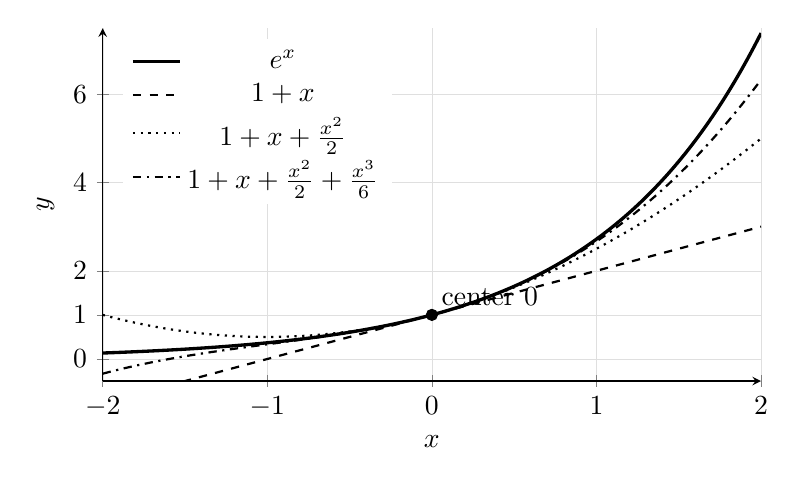
\begin{tikzpicture}
\begin{axis}[
    width=0.82\textwidth,
    height=0.50\textwidth,
    xmin=-2, xmax=2,
    ymin=-0.5, ymax=7.5,
    axis lines=left,
    xlabel={\(x\)},
    ylabel={\(y\)},
    xtick={-2,-1,0,1,2},
    ytick={0,1,2,4,6},
    grid=both,
    grid style={line width=.1pt, draw=gray!25},
    legend style={draw=none, at={(0.03,0.97)}, anchor=north west}
]
\addplot[very thick, domain=-2:2, samples=200] {exp(x)};
\addlegendentry{\(e^x\)}

\addplot[thick, dashed, domain=-2:2, samples=2] {1+x};
\addlegendentry{\(1+x\)}

\addplot[thick, dotted, domain=-2:2, samples=200] {1+x+x^2/2};
\addlegendentry{\(1+x+\frac{x^2}{2}\)}

\addplot[thick, dashdotted, domain=-2:2, samples=200] {1+x+x^2/2+x^3/6};
\addlegendentry{\(1+x+\frac{x^2}{2}+\frac{x^3}{6}\)}

\addplot[only marks, mark=*] coordinates {(0,1)};
\node[anchor=south west] at (axis cs:0,1) {center \(0\)};
\end{axis}
\end{tikzpicture}
\caption{Taylor polynomials for \(e^x\) match more derivatives at the center \(0\).}
\label{fig:taylor-polynomials-exp}
\end{figure}

The polynomials

\[
1,
\qquad
1+x,
\qquad
1+x+\frac{x^2}{2},
\qquad
1+x+\frac{x^2}{2}+\frac{x^3}{6}
\]

are not random.  Each one matches more local information about \(e^x\) at \(0\).

\begin{center}
\begin{tabular}{c|c}
\textbf{polynomial} & \textbf{what it matches at \(0\)} \\ \hline
\(P_0\) & value \\
\(P_1\) & value and first derivative \\
\(P_2\) & value, first derivative, and second derivative \\
\(P_3\) & value through third derivative
\end{tabular}
\end{center}

This is the pattern Taylor polynomials formalize.

\subsection{Linear, quadratic, and cubic approximations}
\label{subsec:linear-quadratic-cubic-approximations}

The first Taylor polynomial is the tangent line:

\[
\boxed{
P_1(x)=f(a)+f'(a)(x-a).
}
\]

It matches \(f\) and \(f'\) at \(a\).

The second Taylor polynomial adds curvature information:

\[
\boxed{
P_2(x)
=
f(a)+f'(a)(x-a)+\frac{f''(a)}{2}(x-a)^2.
}
\]

The third Taylor polynomial adds the third derivative:

\[
\boxed{
P_3(x)
=
f(a)+f'(a)(x-a)
+\frac{f''(a)}{2}(x-a)^2
+\frac{f'''(a)}{6}(x-a)^3.
}
\]

The numbers \(2\) and \(6\) are

\[
2!=2,
\qquad
3!=6.
\]

\paragraph{Example: approximating a square root.}
Find the cubic Taylor polynomial for

\[
f(x)=\sqrt{1+x}
\]

centered at \(0\), and use it to approximate

\[
\sqrt{1.1}.
\]

First compute derivatives:

\[
f(x)=(1+x)^{1/2},
\]

\[
f'(x)=\frac12(1+x)^{-1/2},
\]

\[
f''(x)=-\frac14(1+x)^{-3/2},
\]

\[
f'''(x)=\frac38(1+x)^{-5/2}.
\]

At \(x=0\),

\[
f(0)=1,
\qquad
f'(0)=\frac12,
\qquad
f''(0)=-\frac14,
\qquad
f'''(0)=\frac38.
\]

Therefore

\[
P_3(x)
=
1+\frac12x+\frac{-\frac14}{2}x^2+\frac{\frac38}{6}x^3.
\]

So

\[
\boxed{
P_3(x)=1+\frac{x}{2}-\frac{x^2}{8}+\frac{x^3}{16}.
}
\]

To approximate \(\sqrt{1.1}\), use

\[
1.1=1+0.1.
\]

So \(x=0.1\).  Then

\[
P_3(0.1)
=
1+\frac{0.1}{2}-\frac{(0.1)^2}{8}+\frac{(0.1)^3}{16}.
\]

Compute:

\[
P_3(0.1)
=
1+0.05-0.00125+0.0000625
=
1.0488125.
\]

Thus

\[
\boxed{
\sqrt{1.1}\approx 1.0488125.
}
\]

The approximation is good because \(0.1\) is close to the center \(0\).  The polynomial
was built for nearby inputs.

\paragraph{What each term is doing.}
The approximation

\[
1+\frac{x}{2}
\]

uses the tangent line.  It says that near \(0\),

\[
\sqrt{1+x}
\]

initially rises at rate \(1/2\).

The term

\[
-\frac{x^2}{8}
\]

corrects for concavity.  The square-root graph bends downward, so the tangent line
slightly overestimates.  The negative quadratic term pulls the approximation down.

The term

\[
\frac{x^3}{16}
\]

makes a smaller correction to the correction.

A Taylor polynomial is not just a formula.  Each coefficient records derivative
information at the center.

\subsection{Taylor polynomial centered at \texorpdfstring{\(a\)}{a}}
\label{subsec:taylor-polynomial-centered-at-a}

Now write the general formula.

Suppose \(f\) has derivatives up to order \(n\) at \(x=a\).  The degree \(n\) Taylor
polynomial for \(f\) centered at \(a\) is

\[
\boxed{
T_n(x)
=
f(a)
+
f'(a)(x-a)
+
\frac{f''(a)}{2!}(x-a)^2
+
\cdots
+
\frac{f^{(n)}(a)}{n!}(x-a)^n.
}
\]

In sigma notation,

\[
\boxed{
T_n(x)=
\sum_{k=0}^{n}
\frac{f^{(k)}(a)}{k!}(x-a)^k.
}
\]

Here

\[
f^{(0)}(a)=f(a),
\qquad
0!=1.
\]

\paragraph{Why the coefficients have this form.}
Suppose

\[
P(x)=A_0+A_1(x-a)+A_2(x-a)^2+\cdots+A_n(x-a)^n.
\]

Evaluate at \(x=a\).  Every term with a factor \((x-a)\) disappears, so

\[
P(a)=A_0.
\]

Differentiate once:

\[
P'(x)=A_1+2A_2(x-a)+3A_3(x-a)^2+\cdots.
\]

At \(x=a\),

\[
P'(a)=A_1.
\]

Differentiate twice:

\[
P''(a)=2!A_2.
\]

Differentiate \(k\) times.  At \(x=a\), the only surviving contribution to the \(k\)-th
derivative comes from

\[
A_k(x-a)^k.
\]

It gives

\[
P^{(k)}(a)=k!A_k.
\]

To make \(P^{(k)}(a)=f^{(k)}(a)\), we must choose

\[
A_k=\frac{f^{(k)}(a)}{k!}.
\]

That is exactly the Taylor coefficient.

\paragraph{Example: \(\ln x\) centered at \(1\).}
The logarithm is not defined at \(0\), so a polynomial centered at \(0\) would be a bad
idea.  But \(\ln x\) behaves nicely near \(x=1\).

Let

\[
f(x)=\ln x.
\]

Then

\[
f(1)=0,
\]

\[
f'(x)=\frac1x,
\qquad
f'(1)=1,
\]

\[
f''(x)=-\frac1{x^2},
\qquad
f''(1)=-1,
\]

\[
f'''(x)=\frac2{x^3},
\qquad
f'''(1)=2.
\]

The cubic Taylor polynomial centered at \(1\) is

\[
T_3(x)
=
0+1(x-1)+\frac{-1}{2!}(x-1)^2+\frac{2}{3!}(x-1)^3.
\]

So

\[
\boxed{
T_3(x)
=
(x-1)-\frac{(x-1)^2}{2}+\frac{(x-1)^3}{3}.
}
\]

To approximate \(\ln(1.2)\), use \(x=1.2\).  Then \(x-1=0.2\), and

\[
T_3(1.2)
=
0.2-\frac{(0.2)^2}{2}+\frac{(0.2)^3}{3}.
\]

So

\[
T_3(1.2)
=
0.2-0.02+\frac{0.008}{3}
=
0.182666\ldots.
\]

This matches the earlier logarithm series in another language.  If we write

\[
u=x-1,
\]

then

\[
\ln x=\ln(1+u)
\]

and the polynomial becomes

\[
u-\frac{u^2}{2}+\frac{u^3}{3}.
\]

The center changed the notation, but not the idea.

\subsection{Maclaurin polynomials}
\label{subsec:maclaurin-polynomials}

A Taylor polynomial centered at \(0\) has a special name.

\begin{quote}
\textbf{Maclaurin polynomial.}
The degree \(n\) Taylor polynomial centered at \(0\) is called the degree \(n\)
\emph{Maclaurin polynomial}:

\[
\boxed{
M_n(x)=
\sum_{k=0}^{n}
\frac{f^{(k)}(0)}{k!}x^k.
}
\]
\end{quote}

Many of the most familiar series begin as Maclaurin polynomials.

\paragraph{Example: \(e^x\).}
All derivatives of \(e^x\) are \(e^x\), and

\[
e^0=1.
\]

So every derivative at \(0\) equals \(1\).  Therefore

\[
\boxed{
M_n(x)=
1+x+\frac{x^2}{2!}+\frac{x^3}{3!}+\cdots+\frac{x^n}{n!}
}
\]

for \(e^x\).

\paragraph{Example: \(\sin x\).}
The derivatives of \(\sin x\) cycle:

\[
\sin x,\quad \cos x,\quad -\sin x,\quad -\cos x,\quad \sin x,\ldots.
\]

At \(x=0\),

\[
\sin0=0,
\qquad
\cos0=1.
\]

So the derivatives at \(0\) follow the pattern

\[
0,\ 1,\ 0,\ -1,\ 0,\ 1,\ldots.
\]

Thus the degree \(5\) Maclaurin polynomial is

\[
\boxed{
M_5(x)=x-\frac{x^3}{3!}+\frac{x^5}{5!}.
}
\]

\paragraph{Example: \(\cos x\).}
For \(\cos x\), the derivative values at \(0\) are

\[
1,\ 0,\ -1,\ 0,\ 1,\ 0,\ -1,\ldots.
\]

So the degree \(6\) Maclaurin polynomial is

\[
\boxed{
M_6(x)=1-\frac{x^2}{2!}+\frac{x^4}{4!}-\frac{x^6}{6!}.
}
\]

\begin{center}
\begin{tabular}{c|c}
\textbf{function} & \textbf{early Maclaurin polynomials} \\ \hline
\(e^x\) &
\(1,\quad 1+x,\quad 1+x+\dfrac{x^2}{2!},\quad
1+x+\dfrac{x^2}{2!}+\dfrac{x^3}{3!}\) \\[8pt]
\(\sin x\) &
\(x,\quad x-\dfrac{x^3}{3!},\quad x-\dfrac{x^3}{3!}+\dfrac{x^5}{5!}\) \\[8pt]
\(\cos x\) &
\(1,\quad 1-\dfrac{x^2}{2!},\quad
1-\dfrac{x^2}{2!}+\dfrac{x^4}{4!}\)
\end{tabular}
\end{center}

These are still finite polynomials.  We have not yet proved that the corresponding
infinite series equal the functions.  That distinction matters.

\paragraph{A necessary warning.}
Taylor polynomials require derivatives at the center.

The function

\[
f(x)=|x|
\]

is continuous at \(0\), but it is not differentiable at \(0\).  The left slope is \(-1\), and
the right slope is \(1\).  There is no single number \(f'(0)\).

So there is no first-degree Taylor polynomial for \(|x|\) centered at \(0\) that matches
the derivative.  The needed local data does not exist.

\begin{quote}
\textbf{Moral.}
A Taylor polynomial is built from derivatives at a center.  If those derivatives do not
exist, the polynomial cannot be built in the usual way.
\end{quote}

There is another warning.  Even when the polynomial exists, it is only a local
approximation until we understand its error.

For \(e^x\), the polynomial

\[
1+x+\frac{x^2}{2}
\]

is good near \(0\).  It is not automatically good far away.  Taylor polynomials are
promises about contact at a point, not yet promises about accuracy on a whole interval.

That is the next question:

\[
\boxed{
\text{How far is \(f(x)\) from its Taylor polynomial?}
}
\]

The answer is the remainder term.  Without it, approximation has no scale.

\section{Taylor's theorem and remainders}
\label{sec:taylor-theorem-remainders}

Taylor polynomials gave us a finite approximation:

\[
f(x)\approx T_n(x).
\]

But approximation without an error term is only a hope.  The next question is the one
calculus must answer:

\[
\boxed{
\text{How far is \(f(x)\) from its Taylor polynomial?}
}
\]

The difference

\[
f(x)-T_n(x)
\]

is called the \emph{remainder}.  It is the part of the function that the polynomial has
not yet captured.

\subsection{The error term matters}
\label{subsec:error-term-matters}

For \(f(x)=e^x\), the cubic Maclaurin polynomial is

\[
T_3(x)=1+x+\frac{x^2}{2!}+\frac{x^3}{3!}.
\]

At \(x=1\),

\[
T_3(1)=1+1+\frac12+\frac16=\frac83.
\]

So

\[
e\approx \frac83\approx2.6667.
\]

This is a reasonable first approximation, but the important question is not whether it
looks reasonable.  The important question is:

\[
\text{How large can the error be?}
\]

Define

\[
R_3(1)=e^1-T_3(1).
\]

Then

\[
e=T_3(1)+R_3(1).
\]

The polynomial gives the part we can compute easily.  The remainder tells how much
we may be missing.

\begin{figure}[h]
\centering
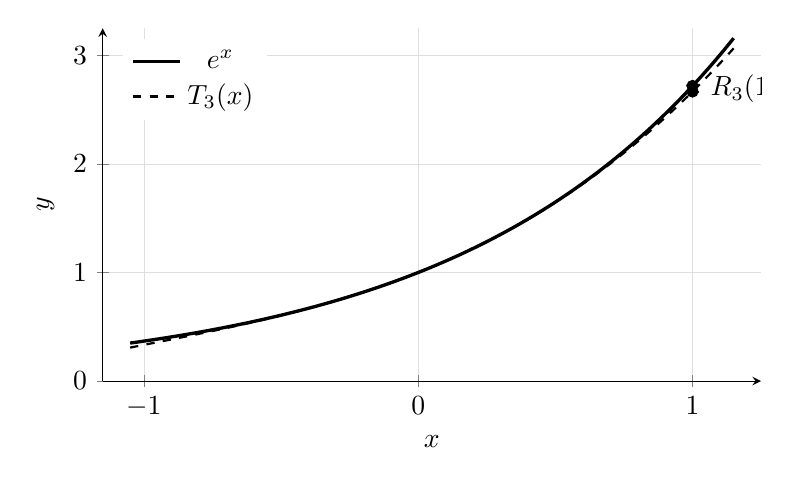
\begin{tikzpicture}
\begin{axis}[
    width=0.82\textwidth,
    height=0.50\textwidth,
    xmin=-1.15, xmax=1.25,
    ymin=0, ymax=3.25,
    axis lines=left,
    xlabel={\(x\)},
    ylabel={\(y\)},
    xtick={-1,0,1},
    ytick={0,1,2,3},
    grid=both,
    grid style={line width=.1pt, draw=gray!25},
    legend style={draw=none, at={(0.03,0.97)}, anchor=north west}
]
\addplot[very thick, domain=-1.05:1.15, samples=200] {exp(x)};
\addlegendentry{\(e^x\)}

\addplot[thick, dashed, domain=-1.05:1.15, samples=200] {1+x+x^2/2+x^3/6};
\addlegendentry{\(T_3(x)\)}

\draw[<->, thick] (axis cs:1,2.6666667) -- (axis cs:1,2.7182818);
\node[anchor=west] at (axis cs:1.03,2.69) {\(R_3(1)\)};
\addplot[only marks, mark=*] coordinates {(1,2.7182818) (1,2.6666667)};
\end{axis}
\end{tikzpicture}
\caption{The remainder is the vertical gap between the function and its Taylor polynomial at the chosen input.}
\label{fig:taylor-remainder-gap}
\end{figure}

For a general function \(f\), centered at \(a\), the degree \(n\) Taylor polynomial is

\[
T_n(x)=
\sum_{k=0}^{n}
\frac{f^{(k)}(a)}{k!}(x-a)^k.
\]

The remainder is

\[
\boxed{
R_n(x)=f(x)-T_n(x).
}
\]

So Taylor's formula is

\[
\boxed{
f(x)=T_n(x)+R_n(x).
}
\]

This equation is exact.  The approximation happens only when we ignore or estimate
\(R_n(x)\).

\begin{quote}
\textbf{Taylor approximation and Taylor formula.}

\[
f(x)\approx T_n(x)
\]

is an approximation.

\[
f(x)=T_n(x)+R_n(x)
\]

is an exact formula.
\end{quote}

The rest of this section is about estimating \(R_n(x)\).

\subsection{Lagrange form of the remainder}
\label{subsec:lagrange-remainder}

The first useful form of the remainder looks surprisingly like the next Taylor term.

For a degree \(n\) Taylor polynomial, the next possible power is

\[
(x-a)^{n+1}.
\]

Taylor's theorem says that the error is exactly this power multiplied by the
\((n+1)\)-st derivative at some point between \(a\) and \(x\).

\begin{quote}
\textbf{Taylor's Theorem with Lagrange remainder.}
Suppose \(f\) has continuous derivatives through order \(n+1\) on an interval containing
\(a\) and \(x\).  Then

\[
\boxed{
f(x)=
\sum_{k=0}^{n}
\frac{f^{(k)}(a)}{k!}(x-a)^k
+
\frac{f^{(n+1)}(c)}{(n+1)!}(x-a)^{n+1}
}
\]

for some number \(c\) between \(a\) and \(x\).

Equivalently,

\[
\boxed{
R_n(x)=
\frac{f^{(n+1)}(c)}{(n+1)!}(x-a)^{n+1}
}
\]

for some \(c\) between \(a\) and \(x\).
\end{quote}

The theorem does not usually tell us the exact value of \(c\).  That is fine.  For error
bounds, we usually do not need \(c\).  We only need a bound on the derivative.

If

\[
|f^{(n+1)}(t)|\le M
\]

for all \(t\) between \(a\) and \(x\), then

\[
\boxed{
|R_n(x)|
\le
\frac{M}{(n+1)!}|x-a|^{n+1}.
}
\]

This is the main practical form.

\paragraph{Example: bounding the error in \(e\).}
Use the degree \(7\) Maclaurin polynomial for \(e^x\) to approximate \(e\).

The polynomial is

\[
T_7(x)
=
1+x+\frac{x^2}{2!}+\frac{x^3}{3!}
+\frac{x^4}{4!}+\frac{x^5}{5!}
+\frac{x^6}{6!}+\frac{x^7}{7!}.
\]

At \(x=1\),

\[
T_7(1)=
1+1+\frac12+\frac16+\frac1{24}+\frac1{120}+\frac1{720}+\frac1{5040}.
\]

So

\[
T_7(1)\approx 2.718254.
\]

Now estimate the error.  Since every derivative of \(e^x\) is \(e^x\), the Lagrange
remainder is

\[
R_7(1)=\frac{e^c}{8!}
\]

for some \(c\) between \(0\) and \(1\).

On this interval,

\[
e^c<3.
\]

Therefore

\[
|R_7(1)|<\frac3{8!}.
\]

Since

\[
8!=40320,
\]

we get

\[
|R_7(1)|<\frac3{40320}<0.000075.
\]

Thus

\[
\boxed{
e=2.718254\ldots \quad \text{with error less than }0.000075.
}
\]

The approximation is not just a decimal.  It comes with a guarantee.

\paragraph{Example: a sine approximation.}
Approximate

\[
\sin(0.5)
\]

using

\[
\sin x\approx x-\frac{x^3}{3!}.
\]

This is the fourth-degree Maclaurin polynomial too, because the \(x^4\) coefficient is
zero:

\[
T_4(x)=x-\frac{x^3}{3!}.
\]

Taylor's theorem gives

\[
R_4(x)=\frac{f^{(5)}(c)}{5!}x^5
\]

for some \(c\) between \(0\) and \(x\).  For \(f(x)=\sin x\), the fifth derivative is

\[
f^{(5)}(x)=\cos x.
\]

Thus

\[
|f^{(5)}(c)|=|\cos c|\le1.
\]

So

\[
|R_4(x)|\le \frac{|x|^5}{5!}.
\]

At \(x=0.5\),

\[
|R_4(0.5)|\le \frac{(0.5)^5}{120}.
\]

Since

\[
(0.5)^5=\frac1{32},
\]

we have

\[
|R_4(0.5)|\le \frac1{3840}<0.0003.
\]

The approximation is

\[
0.5-\frac{(0.5)^3}{6}
=
0.5-\frac{0.125}{6}
=
0.479166\ldots.
\]

Therefore

\[
\boxed{
\sin(0.5)\approx0.479166
}
\]

with error less than \(0.0003\).

\begin{quote}
\textbf{What controls the error?}

The bound

\[
|R_n(x)|\le
\frac{M}{(n+1)!}|x-a|^{n+1}
\]

has three ingredients:

\begin{center}
\begin{tabular}{c|l}
\textbf{ingredient} & \textbf{meaning} \\ \hline
\(M\) & how large the next derivative can be \\
\(|x-a|^{n+1}\) & how far \(x\) is from the center \\
\((n+1)!\) & how strongly higher degree terms are divided down
\end{tabular}
\end{center}
\end{quote}

This explains why Taylor polynomials are local.  If \(x\) is close to \(a\), the factor

\[
|x-a|^{n+1}
\]

is small.  If \(x\) is far from \(a\), the same polynomial may lose accuracy.

\paragraph{A local warning.}
For

\[
\frac1{1-x},
\]

the Maclaurin polynomials are

\[
1+x+x^2+\cdots+x^n.
\]

At \(x=\frac12\), these polynomials approach

\[
\frac1{1-\frac12}=2.
\]

But at \(x=2\), the same partial sums are

\[
1+2+2^2+\cdots+2^n,
\]

which do not approach

\[
\frac1{1-2}=-1.
\]

The problem is not the function.  The function is defined at \(x=2\).  The problem is
that the power series centered at \(0\) has radius \(1\).  A Taylor polynomial is built
from local information.  It should not be trusted far from its center without an error
estimate.

\subsection{Proof idea for Taylor's theorem}
\label{subsec:proof-idea-taylor-theorem}

Taylor's theorem is a higher-order version of the Mean Value Theorem.

For \(n=0\), Taylor's theorem says

\[
f(x)=f(a)+f'(c)(x-a)
\]

for some \(c\) between \(a\) and \(x\).  This is exactly the Mean Value Theorem.

For larger \(n\), the idea is to subtract off a polynomial that matches \(f\) at \(a\) as
closely as possible, then apply Rolle's Theorem repeatedly.

Here is the proof.

Assume \(x\neq a\), and let

\[
T_n(t)=
\sum_{k=0}^{n}
\frac{f^{(k)}(a)}{k!}(t-a)^k.
\]

Define

\[
K=\frac{f(x)-T_n(x)}{(x-a)^{n+1}}.
\]

Now build the auxiliary function

\[
\Phi(t)=f(t)-T_n(t)-K(t-a)^{n+1}.
\]

This function is designed so that

\[
\Phi(x)=0.
\]

It also satisfies

\[
\Phi(a)=0.
\]

Even more is true.  Since \(T_n\) matches \(f\) and its first \(n\) derivatives at \(a\),

\[
\Phi(a)=\Phi'(a)=\Phi''(a)=\cdots=\Phi^{(n)}(a)=0.
\]

The function \(\Phi\) has zeros at \(a\) and \(x\).  By Rolle's Theorem, \(\Phi'\) has a
zero between \(a\) and \(x\).  Since \(\Phi'(a)=0\), Rolle's Theorem can be applied
again to \(\Phi'\).  Repeating this idea \(n+1\) times gives a point \(c\) between \(a\)
and \(x\) such that

\[
\Phi^{(n+1)}(c)=0.
\]

Now compute \(\Phi^{(n+1)}\).  The polynomial \(T_n\) has degree \(n\), so its
\((n+1)\)-st derivative is \(0\).  Also,

\[
\frac{d^{\,n+1}}{dt^{n+1}}(t-a)^{n+1}=(n+1)!.
\]

Thus

\[
\Phi^{(n+1)}(t)=f^{(n+1)}(t)-K(n+1)!.
\]

At \(t=c\),

\[
0=f^{(n+1)}(c)-K(n+1)!.
\]

Therefore

\[
K=\frac{f^{(n+1)}(c)}{(n+1)!}.
\]

Since

\[
f(x)-T_n(x)=K(x-a)^{n+1},
\]

we get

\[
f(x)-T_n(x)
=
\frac{f^{(n+1)}(c)}{(n+1)!}(x-a)^{n+1}.
\]

This is the Lagrange remainder.

\begin{quote}
\textbf{Why Rolle's Theorem appears.}
The Taylor polynomial makes the function and polynomial agree at \(a\) through many
derivatives.  After subtracting them, we get many zeros at \(a\).  Rolle's Theorem turns
many zeros into information about a higher derivative.
\end{quote}

\subsection{Integral form of the remainder}
\label{subsec:integral-form-remainder}

The Lagrange form is excellent for error bounds.  There is another form that shows the
accumulation structure more clearly.

\begin{quote}
\textbf{Integral form of the Taylor remainder.}
If \(f^{(n+1)}\) is continuous on an interval containing \(a\) and \(x\), then

\[
\boxed{
R_n(x)=
\int_a^x
\frac{f^{(n+1)}(t)}{n!}(x-t)^n\,dt.
}
\]
\end{quote}

This says that the error is accumulated from the next derivative, with a weight

\[
\frac{(x-t)^n}{n!}.
\]

For \(n=0\), the formula becomes

\[
R_0(x)=\int_a^x f'(t)\,dt.
\]

Since

\[
R_0(x)=f(x)-f(a),
\]

this is just the Fundamental Theorem:

\[
f(x)-f(a)=\int_a^x f'(t)\,dt.
\]

So the integral remainder is a higher-order version of the same accumulation idea.

\paragraph{Example: the first few cases.}
For \(n=1\),

\[
f(x)=f(a)+f'(a)(x-a)+\int_a^x f''(t)(x-t)\,dt.
\]

For \(n=2\),

\[
f(x)=f(a)+f'(a)(x-a)+\frac{f''(a)}{2}(x-a)^2
+\int_a^x \frac{f'''(t)}{2}(x-t)^2\,dt.
\]

The pattern is visible.  The Taylor polynomial uses derivative information at the center.
The remainder accumulates the next derivative over the interval.

\paragraph{Why the formula is true.}
Start with the Fundamental Theorem:

\[
f(x)-f(a)=\int_a^x f'(t)\,dt.
\]

Now integrate by parts with

\[
u=f'(t),
\qquad
dv=dt.
\]

A more useful repeated version is this: each integration by parts pulls out one Taylor
term at \(a\), and leaves an integral involving one higher derivative.

For example,

\[
\int_a^x f''(t)(x-t)\,dt
=
f(x)-f(a)-f'(a)(x-a).
\]

Rearranging gives

\[
f(x)=f(a)+f'(a)(x-a)+\int_a^x f''(t)(x-t)\,dt.
\]

Repeating the same step gives the general formula.

This form is optional for computation, but important for the story.  Taylor's theorem is
not magic.  The error is an accumulated effect of higher derivatives.

\subsection{Alternating-series remainders as a special case}
\label{subsec:alternating-series-remainders-special-case}

Some Taylor series are alternating series.  When the term sizes decrease to \(0\), the
Alternating Series Estimation Theorem gives a very simple error bound:

\[
\boxed{
\text{error} \le \text{first omitted term in absolute value}.
}
\]

This often gives a sharper and easier estimate than the Lagrange bound.

From Section \ref{subsec:series-for-arctan}, we found

\[
\arctan x
=
x-\frac{x^3}{3}+\frac{x^5}{5}-\frac{x^7}{7}+\cdots,
\qquad |x|\le1.
\]

For \(0<x\le1\), the terms alternate and decrease in size.  Therefore, if we stop after

\[
x-\frac{x^3}{3}+\frac{x^5}{5},
\]

then the error is at most

\[
\frac{x^7}{7}.
\]

\paragraph{Example: estimating \(\arctan(1/2)\).}
Use

\[
\arctan x
\approx
x-\frac{x^3}{3}+\frac{x^5}{5}.
\]

At \(x=\frac12\),

\[
\arctan\frac12
\approx
\frac12-\frac{1}{3\cdot2^3}+\frac{1}{5\cdot2^5}.
\]

Compute:

\[
\frac12-\frac1{24}+\frac1{160}
=
0.464583\ldots.
\]

The first omitted term has size

\[
\frac{(1/2)^7}{7}
=
\frac1{7\cdot128}
=
\frac1{896}.
\]

So

\[
\boxed{
\left|
\arctan\frac12-0.464583\ldots
\right|
\le
\frac1{896}
<0.0012.
}
\]

Since the first omitted term is negative, the true value is slightly less than the
partial sum.

\paragraph{Example: estimating \(\ln(1.1)\).}
From Section \ref{subsec:series-for-log-one-plus-x},

\[
\ln(1+x)
=
x-\frac{x^2}{2}+\frac{x^3}{3}-\frac{x^4}{4}+\cdots
\]

for \(-1<x\le1\).  At \(x=0.1\), use four terms:

\[
\ln(1.1)
\approx
0.1-\frac{0.1^2}{2}+\frac{0.1^3}{3}-\frac{0.1^4}{4}.
\]

The first omitted term has size

\[
\frac{0.1^5}{5}=0.000002.
\]

Thus

\[
\boxed{
\left|
\ln(1.1)
-
\left(
0.1-\frac{0.1^2}{2}+\frac{0.1^3}{3}-\frac{0.1^4}{4}
\right)
\right|
\le 0.000002.
}
\]

The input \(0.1\) is small, so the powers shrink quickly.

\begin{quote}
\textbf{Two ways to estimate a Taylor error.}

\begin{center}
\begin{tabular}{c|l}
\textbf{method} & \textbf{when it is useful} \\ \hline
Lagrange remainder & when we can bound the next derivative \\[3pt]
Alternating estimate & when the Taylor terms alternate and decrease
\end{tabular}
\end{center}
\end{quote}

Taylor's theorem gives finite approximations with controlled error.  The next step is to
let the degree grow without bound.  If the remainders tend to \(0\), the Taylor
polynomials become a Taylor series for the function.

\section{Taylor series for elementary functions}
\label{sec:taylor-series-elementary-functions}

Taylor's theorem says

\[
f(x)=T_n(x)+R_n(x).
\]

If the remainders satisfy

\[
R_n(x)\to0
\]

as \(n\to\infty\), then the Taylor polynomials approach the function itself:

\[
f(x)=\lim_{n\to\infty}T_n(x).
\]

That limit is an infinite series.

\begin{quote}
\textbf{Taylor series.}
If \(f\) has derivatives of all orders at \(a\), its Taylor series centered at \(a\) is

\[
\boxed{
\sum_{n=0}^{\infty}
\frac{f^{(n)}(a)}{n!}(x-a)^n.
}
\]

When \(a=0\), this is called the Maclaurin series:

\[
\boxed{
\sum_{n=0}^{\infty}
\frac{f^{(n)}(0)}{n!}x^n.
}
\]
\end{quote}

There is a warning hidden in the definition.  The Taylor series is built from the
derivatives of \(f\) at one point.  It may converge only for some \(x\)-values.  Even when
it converges, it must still be checked that it converges to \(f(x)\).

\[
\boxed{
\text{A Taylor series equals the function only where the remainder tends to \(0\).}
}
\]

For the elementary functions in this section, we will prove or recall why the equality
is valid.

\subsection{\texorpdfstring{\(e^x\)}{e^x}}
\label{subsec:taylor-series-exp}

The exponential function is the cleanest Taylor series because every derivative is the
same:

\[
\frac{d^n}{dx^n}e^x=e^x.
\]

At \(x=0\),

\[
e^0=1.
\]

So

\[
f^{(n)}(0)=1
\]

for every \(n\).  The Maclaurin series is therefore

\[
\boxed{
e^x
=
1+x+\frac{x^2}{2!}+\frac{x^3}{3!}
+\frac{x^4}{4!}+\cdots
}
\]

or

\[
\boxed{
e^x=\sum_{n=0}^{\infty}\frac{x^n}{n!}.
}
\]

Now we justify the equality.

The degree \(n\) Maclaurin polynomial is

\[
T_n(x)=\sum_{k=0}^{n}\frac{x^k}{k!}.
\]

Taylor's theorem gives

\[
R_n(x)=\frac{e^c}{(n+1)!}x^{n+1}
\]

for some \(c\) between \(0\) and \(x\).  For a fixed \(x\), the value \(e^c\) is bounded.
For example,

\[
e^c\le e^{|x|}
\]

for \(c\) between \(0\) and \(x\).  Therefore

\[
|R_n(x)|
\le
e^{|x|}\frac{|x|^{n+1}}{(n+1)!}.
\]

The factor

\[
\frac{|x|^{n+1}}{(n+1)!}
\]

tends to \(0\), because factorials eventually grow faster than any fixed power.  Thus

\[
R_n(x)\to0
\]

for every real \(x\).

So the exponential series is valid for all real \(x\):

\[
\boxed{
e^x=\sum_{n=0}^{\infty}\frac{x^n}{n!},
\qquad -\infty<x<\infty.
}
\]

\paragraph{Example: estimating \(e^{0.3}\).}
Use terms through \(x^4\):

\[
e^{0.3}
\approx
1+0.3+\frac{0.3^2}{2!}+\frac{0.3^3}{3!}+\frac{0.3^4}{4!}.
\]

Compute:

\[
1+0.3+0.045+0.0045+0.0003375
=
1.3498375.
\]

The remainder after degree \(4\) is

\[
R_4(0.3)=\frac{e^c}{5!}(0.3)^5
\]

for some \(c\) between \(0\) and \(0.3\).  Since \(e^c<2\) on this interval,

\[
|R_4(0.3)|<\frac{2(0.3)^5}{120}.
\]

Now

\[
(0.3)^5=0.00243,
\]

so

\[
|R_4(0.3)|<0.000041.
\]

Thus

\[
\boxed{
e^{0.3}\approx1.3498375
}
\]

with error less than \(0.000041\).

\subsection{\texorpdfstring{\(\sin x\) and \(\cos x\)}{sin x and cos x}}
\label{subsec:taylor-series-sin-cos}

The derivatives of \(\sin x\) cycle:

\[
\sin x,\quad \cos x,\quad -\sin x,\quad -\cos x,\quad \sin x,\ldots.
\]

At \(x=0\),

\[
\sin0=0,
\qquad
\cos0=1.
\]

So the derivative values are

\[
0,\ 1,\ 0,\ -1,\ 0,\ 1,\ 0,\ -1,\ldots.
\]

Only odd powers appear:

\[
\boxed{
\sin x
=
x-\frac{x^3}{3!}+\frac{x^5}{5!}-\frac{x^7}{7!}+\cdots
}
\]

or

\[
\boxed{
\sin x=
\sum_{n=0}^{\infty}
(-1)^n\frac{x^{2n+1}}{(2n+1)!}.
}
\]

For \(\cos x\), the derivative values at \(0\) are

\[
1,\ 0,\ -1,\ 0,\ 1,\ 0,\ -1,\ldots.
\]

Only even powers appear:

\[
\boxed{
\cos x
=
1-\frac{x^2}{2!}+\frac{x^4}{4!}-\frac{x^6}{6!}+\cdots
}
\]

or

\[
\boxed{
\cos x=
\sum_{n=0}^{\infty}
(-1)^n\frac{x^{2n}}{(2n)!}.
}
\]

The equality is valid for all real \(x\).  Here is why.  Every derivative of \(\sin x\) or
\(\cos x\) is one of

\[
\sin x,\quad \cos x,\quad -\sin x,\quad -\cos x.
\]

All of these have absolute value at most \(1\).  Taylor's theorem gives

\[
|R_n(x)|\le \frac{|x|^{n+1}}{(n+1)!}.
\]

For each fixed \(x\), this tends to \(0\).  Therefore the Taylor series for sine and cosine
converge to the functions for every real \(x\).

\[
\boxed{
\sin x=\sum_{n=0}^{\infty}
(-1)^n\frac{x^{2n+1}}{(2n+1)!},
\qquad -\infty<x<\infty,
}
\]

\[
\boxed{
\cos x=\sum_{n=0}^{\infty}
(-1)^n\frac{x^{2n}}{(2n)!},
\qquad -\infty<x<\infty.
}
\]

\begin{figure}[h]
\centering
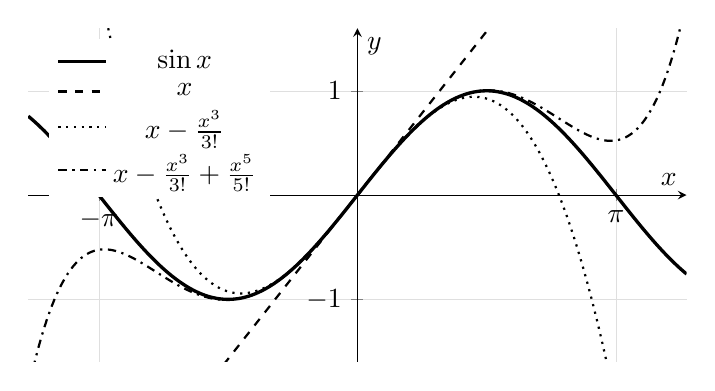
\begin{tikzpicture}
\begin{axis}[
    width=0.82\textwidth,
    height=0.48\textwidth,
    xmin=-4, xmax=4,
    ymin=-1.6, ymax=1.6,
    axis lines=middle,
    xlabel={\(x\)},
    ylabel={\(y\)},
    xtick={-3.1416,0,3.1416},
    xticklabels={\(-\pi\),\(0\),\(\pi\)},
    ytick={-1,0,1},
    grid=both,
    grid style={line width=.1pt, draw=gray!25},
    legend style={draw=none, at={(0.03,0.97)}, anchor=north west}
]
\addplot[very thick, domain=-4:4, samples=250] {sin(deg(x))};
\addlegendentry{\(\sin x\)}

\addplot[thick, dashed, domain=-4:4, samples=250] {x};
\addlegendentry{\(x\)}

\addplot[thick, dotted, domain=-4:4, samples=250] {x-x^3/6};
\addlegendentry{\(x-\frac{x^3}{3!}\)}

\addplot[thick, dashdotted, domain=-4:4, samples=250] {x-x^3/6+x^5/120};
\addlegendentry{\(x-\frac{x^3}{3!}+\frac{x^5}{5!}\)}
\end{axis}
\end{tikzpicture}
\caption{Taylor polynomials for \(\sin x\) are best near the center \(0\), then improve outward as more terms are added.}
\label{fig:sin-taylor-polynomials}
\end{figure}

\paragraph{Example: estimating \(\sin(0.2)\).}
Use

\[
\sin x\approx x-\frac{x^3}{3!}.
\]

At \(x=0.2\),

\[
0.2-\frac{0.2^3}{6}
=
0.2-\frac{0.008}{6}
=
0.198666\ldots.
\]

Because the sine series is alternating with decreasing term sizes for this input, the error
is at most the first omitted term:

\[
\frac{0.2^5}{5!}.
\]

Since

\[
0.2^5=0.00032,
\]

we get

\[
\frac{0.2^5}{120}
=
0.000002666\ldots.
\]

Thus

\[
\boxed{
\sin(0.2)\approx0.198666\ldots
}
\]

with error less than \(0.000003\).

\subsection{\texorpdfstring{\(\ln(1+x)\)}{ln(1+x)}}
\label{subsec:taylor-series-ln-one-plus-x}

The logarithm series was already discovered by integrating the geometric series:

\[
\frac1{1+x}=1-x+x^2-x^3+\cdots,
\qquad |x|<1.
\]

Integrating from \(0\) to \(x\) gave

\[
\ln(1+x)
=
x-\frac{x^2}{2}+\frac{x^3}{3}-\frac{x^4}{4}+\cdots.
\]

Now we see why these are the Taylor coefficients.

Let

\[
f(x)=\ln(1+x).
\]

Then

\[
f(0)=0.
\]

Also,

\[
f'(x)=\frac1{1+x},
\]

\[
f''(x)=-\frac1{(1+x)^2},
\]

\[
f'''(x)=\frac{2}{(1+x)^3}.
\]

The pattern is

\[
f^{(n)}(x)=
(-1)^{n-1}\frac{(n-1)!}{(1+x)^n},
\qquad n\ge1.
\]

At \(x=0\),

\[
f^{(n)}(0)=(-1)^{n-1}(n-1)!.
\]

Therefore the coefficient of \(x^n\) is

\[
\frac{f^{(n)}(0)}{n!}
=
\frac{(-1)^{n-1}(n-1)!}{n!}
=
\frac{(-1)^{n-1}}{n}.
\]

So

\[
\boxed{
\ln(1+x)
=
x-\frac{x^2}{2}+\frac{x^3}{3}-\frac{x^4}{4}+\cdots
}
\]

or

\[
\boxed{
\ln(1+x)=
\sum_{n=1}^{\infty}
(-1)^{n-1}\frac{x^n}{n}.
}
\]

The interval of convergence is

\[
\boxed{(-1,1].}
\]

At \(x=1\), this gives the important identity

\[
\boxed{
\ln2=1-\frac12+\frac13-\frac14+\cdots.
}
\]

At \(x=-1\), the series becomes

\[
-1-\frac12-\frac13-\frac14-\cdots,
\]

which diverges.  This matches the function side: \(\ln(1+x)\) is not defined at
\(x=-1\).

\paragraph{Example: estimating \(\ln(1.2)\).}
Here

\[
1.2=1+0.2,
\]

so \(x=0.2\).  Use four terms:

\[
\ln(1.2)
\approx
0.2-\frac{0.2^2}{2}+\frac{0.2^3}{3}-\frac{0.2^4}{4}.
\]

Compute:

\[
0.2-0.02+\frac{0.008}{3}-\frac{0.0016}{4}
=
0.182266\ldots.
\]

The first omitted term has size

\[
\frac{0.2^5}{5}
=
\frac{0.00032}{5}
=
0.000064.
\]

Therefore

\[
\boxed{
\ln(1.2)\approx0.182266\ldots
}
\]

with error less than \(0.000064\).

The logarithm series is most useful when \(x\) is close to \(0\).  That means the number
inside the logarithm,

\[
1+x,
\]

is close to \(1\).

\subsection{\texorpdfstring{\(\arctan x\)}{arctan x}}
\label{subsec:taylor-series-arctan}

The inverse tangent also came from the geometric series.  Since

\[
\frac{d}{dx}\arctan x=\frac1{1+x^2},
\]

and

\[
\frac1{1+x^2}
=
1-x^2+x^4-x^6+\cdots,
\qquad |x|<1,
\]

integrating from \(0\) to \(x\) gave

\[
\arctan x
=
x-\frac{x^3}{3}+\frac{x^5}{5}-\frac{x^7}{7}+\cdots.
\]

Thus

\[
\boxed{
\arctan x=
\sum_{n=0}^{\infty}
(-1)^n\frac{x^{2n+1}}{2n+1}.
}
\]

The interval of convergence is

\[
\boxed{[-1,1].}
\]

At \(x=1\),

\[
\arctan 1=\frac{\pi}{4},
\]

so

\[
\boxed{
\frac{\pi}{4}
=
1-\frac13+\frac15-\frac17+\cdots.
}
\]

This identity is beautiful, but slow.  The terms shrink like odd reciprocals.  As we saw
earlier, using smaller inputs such as \(1/2\) and \(1/3\) makes the same series much
faster.

\paragraph{Example: estimating \(\arctan(0.1)\).}
Use

\[
\arctan x\approx x-\frac{x^3}{3}.
\]

At \(x=0.1\),

\[
\arctan(0.1)
\approx
0.1-\frac{0.001}{3}
=
0.099666\ldots.
\]

The first omitted term has size

\[
\frac{0.1^5}{5}
=
0.000002.
\]

Therefore

\[
\boxed{
\arctan(0.1)\approx0.099666\ldots
}
\]

with error less than \(0.000002\).

\subsection{Binomial series}
\label{subsec:binomial-series}

The geometric series is one member of a larger family.

For a positive integer \(m\), the binomial theorem says

\[
(1+x)^m
=
\sum_{n=0}^{m}
\binom{m}{n}x^n.
\]

For example,

\[
(1+x)^3=1+3x+3x^2+x^3.
\]

But calculus allows the exponent to be any real number \(p\), not only a nonnegative
integer.  The price is that the polynomial usually becomes an infinite series.

First define the generalized binomial coefficients:

\[
\binom{p}{0}=1,
\]

and, for \(n\ge1\),

\[
\boxed{
\binom{p}{n}
=
\frac{p(p-1)(p-2)\cdots(p-n+1)}{n!}.
}
\]

When \(p\) is a nonnegative integer, this agrees with the usual binomial coefficient,
and the coefficients eventually become zero.

\begin{quote}
\textbf{Binomial series.}
For any real number \(p\),

\[
\boxed{
(1+x)^p
=
\sum_{n=0}^{\infty}
\binom{p}{n}x^n
}
\]

for

\[
\boxed{|x|<1.}
\]

If \(p\) is a nonnegative integer, the series terminates and becomes the ordinary
binomial theorem.
\end{quote}

Written out, the series is

\[
\boxed{
(1+x)^p
=
1+px+\frac{p(p-1)}{2!}x^2
+\frac{p(p-1)(p-2)}{3!}x^3+\cdots.
}
\]

\paragraph{Why this is a Taylor series.}
Let

\[
f(x)=(1+x)^p.
\]

Then

\[
f'(x)=p(1+x)^{p-1},
\]

\[
f''(x)=p(p-1)(1+x)^{p-2},
\]

and in general,

\[
f^{(n)}(x)=p(p-1)\cdots(p-n+1)(1+x)^{p-n}.
\]

At \(x=0\),

\[
f^{(n)}(0)=p(p-1)\cdots(p-n+1).
\]

So the Taylor coefficient is

\[
\frac{f^{(n)}(0)}{n!}
=
\binom{p}{n}.
\]

That gives the formal Taylor series.

\paragraph{Why it converges to \((1+x)^p\) for \(|x|<1\).}
Let

\[
B_p(x)=\sum_{n=0}^{\infty}\binom{p}{n}x^n.
\]

The Ratio Test gives radius of convergence \(1\), unless the series terminates.  Inside
\(|x|<1\), power series can be differentiated term by term.

Differentiate \(B_p\) and multiply by \(1+x\).  A coefficient check gives

\[
(1+x)B_p'(x)=pB_p(x).
\]

Also,

\[
B_p(0)=1.
\]

The function

\[
F(x)=(1+x)^p
\]

satisfies the same equation:

\[
(1+x)F'(x)=pF(x),
\]

and

\[
F(0)=1.
\]

Now compare them by forming

\[
H(x)=\frac{B_p(x)}{(1+x)^p}.
\]

On \(-1<x<1\),

\[
H'(x)=0.
\]

So \(H\) is constant.  Since

\[
H(0)=1,
\]

we get

\[
H(x)=1.
\]

Therefore

\[
B_p(x)=(1+x)^p
\]

for \(|x|<1\).

\paragraph{Example: the square-root series.}
Take

\[
p=\frac12.
\]

Then

\[
(1+x)^{1/2}
=
1+\frac12x+\frac{\frac12(-\frac12)}{2!}x^2
+\frac{\frac12(-\frac12)(-\frac32)}{3!}x^3+\cdots.
\]

So

\[
\boxed{
\sqrt{1+x}
=
1+\frac{x}{2}-\frac{x^2}{8}+\frac{x^3}{16}
-\frac{5x^4}{128}+\cdots,
\qquad |x|<1.
}
\]

This explains the coefficients we found earlier from Taylor polynomials.

\paragraph{Example: estimating \(\sqrt{1.1}\).}
Here

\[
1.1=1+0.1.
\]

Use the terms through \(x^4\):

\[
\sqrt{1.1}
\approx
1+\frac{0.1}{2}-\frac{0.1^2}{8}
+\frac{0.1^3}{16}
-\frac{5(0.1)^4}{128}.
\]

Compute:

\[
1+0.05-0.00125+0.0000625-0.00000390625
=
1.04880859375.
\]

The next term has size

\[
\frac{7}{256}(0.1)^5<0.0000003.
\]

So

\[
\boxed{
\sqrt{1.1}\approx1.048808594
}
\]

with error less than \(0.0000003\).

\paragraph{Recovering the geometric series.}
Take

\[
p=-1.
\]

Then

\[
(1+x)^{-1}
=
1-x+x^2-x^3+\cdots,
\qquad |x|<1.
\]

This is the familiar series

\[
\frac1{1+x}=1-x+x^2-x^3+\cdots.
\]

Replacing \(x\) by \(-x\) gives

\[
\frac1{1-x}=1+x+x^2+x^3+\cdots.
\]

So the geometric series is a binomial series with exponent \(-1\).

\subsection{A table of common Taylor series}
\label{subsec:common-taylor-series-table}

The most common Maclaurin series are worth keeping together.

\begin{center}
\renewcommand{\arraystretch}{1.7}
\begin{tabular}{c|c|c}
\textbf{function} & \textbf{Maclaurin series} & \textbf{where valid} \\ \hline
\(e^x\) &
\(\displaystyle \sum_{n=0}^{\infty}\frac{x^n}{n!}\) &
\((-\infty,\infty)\) \\

\(\sin x\) &
\(\displaystyle \sum_{n=0}^{\infty}(-1)^n\frac{x^{2n+1}}{(2n+1)!}\) &
\((-\infty,\infty)\) \\

\(\cos x\) &
\(\displaystyle \sum_{n=0}^{\infty}(-1)^n\frac{x^{2n}}{(2n)!}\) &
\((-\infty,\infty)\) \\

\(\dfrac1{1-x}\) &
\(\displaystyle \sum_{n=0}^{\infty}x^n\) &
\((-1,1)\) \\

\(\ln(1+x)\) &
\(\displaystyle \sum_{n=1}^{\infty}(-1)^{n-1}\frac{x^n}{n}\) &
\((-1,1]\) \\

\(\arctan x\) &
\(\displaystyle \sum_{n=0}^{\infty}(-1)^n\frac{x^{2n+1}}{2n+1}\) &
\([-1,1]\) \\

\((1+x)^p\) &
\(\displaystyle \sum_{n=0}^{\infty}\binom{p}{n}x^n\) &
\(|x|<1\)
\end{tabular}
\end{center}

For the binomial series, endpoints must be tested separately unless the series
terminates.

\begin{quote}
\textbf{How to use the table.}

A Taylor series is not only a memorized formula.  Each formula has three parts:

\[
\text{function}
\qquad
\text{series}
\qquad
\text{interval where it is valid}.
\]

Leaving out the interval is leaving out part of the mathematics.
\end{quote}

We now have a library of infinite polynomial representations.  The next section turns
that library into a tool for computation: estimating function values, evaluating limits,
approximating integrals, and even solving differential equations by matching
coefficients.

\section{Applications of Taylor series}
\label{sec:applications-taylor-series}

The last section collected Taylor series for the elementary functions:

\[
e^x,\qquad \sin x,\qquad \cos x,\qquad \ln(1+x),\qquad \arctan x,
\qquad (1+x)^p.
\]

These formulas are not only identities.  They are tools.

A Taylor series can turn a difficult function into a polynomial calculation.  That makes
it useful for estimating function values, evaluating limits, approximating integrals, and
solving differential equations.

But the same warning remains:

\[
\boxed{
\text{A Taylor approximation is useful only when its error is controlled.}
}
\]

So every application in this section will keep the error visible.

\subsection{Estimating function values}
\label{subsec:estimating-function-values-taylor}

A calculator gives decimal values quickly.  Taylor series explain where those decimals can
come from.

The basic idea is simple:

\[
\text{replace the function by a polynomial near the center.}
\]

The error estimate tells how many terms are needed.

\paragraph{Example: estimating \(e^{0.2}\).}
Use the Maclaurin series

\[
e^x=
1+x+\frac{x^2}{2!}+\frac{x^3}{3!}+\frac{x^4}{4!}+\cdots.
\]

At \(x=0.2\), terms shrink quickly.  Use terms through degree \(4\):

\[
e^{0.2}
\approx
1+0.2+\frac{0.2^2}{2!}+\frac{0.2^3}{3!}+\frac{0.2^4}{4!}.
\]

Compute:

\[
1+0.2+0.02+\frac{0.008}{6}+\frac{0.0016}{24}
=
1.2214.
\]

Now bound the error.  Taylor's theorem gives

\[
R_4(0.2)=\frac{e^c}{5!}(0.2)^5
\]

for some \(c\) between \(0\) and \(0.2\).  Since

\[
e^c<2
\]

on this interval,

\[
|R_4(0.2)|
<
\frac{2(0.2)^5}{5!}.
\]

Because

\[
(0.2)^5=0.00032
\qquad\text{and}\qquad
5!=120,
\]

we get

\[
|R_4(0.2)|<0.000006.
\]

Therefore

\[
\boxed{
e^{0.2}\approx1.2214
}
\]

with error less than \(0.000006\).

The decimal is not just a guess.  It has a guarantee.

\paragraph{Example: estimating \(\sin(0.5)\) to six decimal places.}
The sine series is

\[
\sin x=
x-\frac{x^3}{3!}+\frac{x^5}{5!}-\frac{x^7}{7!}+\cdots.
\]

At \(x=0.5\), the series is alternating and the term sizes decrease.  To get six decimal
places, we want the error less than about

\[
0.000001.
\]

If we stop after the \(x^5\) term, the first omitted term has size

\[
\frac{0.5^7}{7!}
=
\frac{0.0078125}{5040}
>
0.000001.
\]

So include the \(x^7\) term.  Then the first omitted term has size

\[
\frac{0.5^9}{9!}
<0.000000006.
\]

Thus

\[
\sin(0.5)
\approx
0.5-\frac{0.5^3}{3!}
+\frac{0.5^5}{5!}
-\frac{0.5^7}{7!}.
\]

Compute:

\[
0.5-\frac{0.125}{6}
+\frac{0.03125}{120}
-\frac{0.0078125}{5040}
=
0.4794255\ldots.
\]

So

\[
\boxed{
\sin(0.5)\approx0.479426
}
\]

to six decimal places.

\begin{quote}
\textbf{Radian warning.}
The Taylor series for \(\sin x\) and \(\cos x\) use radians.  The approximation

\[
\sin x\approx x
\]

near \(0\) is true when \(x\) is measured in radians, not degrees.
\end{quote}

\paragraph{Choosing the center.}
Taylor series work best near their center.

To estimate

\[
e^{3.02},
\]

the Maclaurin series for \(e^x\) would converge, but the input \(3.02\) is not small.
A better idea is to write

\[
e^{3.02}=e^3e^{0.02}.
\]

Then the Taylor series is used only on

\[
e^{0.02},
\]

where the powers of \(0.02\) shrink very quickly.

This is a general strategy:

\[
\boxed{
\text{move the hard part into a known value and use Taylor series on a small remainder.}
}
\]

For logarithms, this often means rewriting the input so that it is close to \(1\).  For
trigonometric functions, it often means using symmetry or periodicity to reduce the
angle.

\begin{center}
\renewcommand{\arraystretch}{1.4}
\begin{tabular}{c|c|c}
\textbf{function} & \textbf{series center} & \textbf{best inputs} \\ \hline
\(e^x\) & \(0\) & \(x\) close to \(0\) \\
\(\sin x,\cos x\) & \(0\) & angles close to \(0\), in radians \\
\(\ln(1+x)\) & \(0\) & \(1+x\) close to \(1\) \\
\(\arctan x\) & \(0\) & \(x\) close to \(0\) \\
\((1+x)^p\) & \(0\) & \(1+x\) close to \(1\)
\end{tabular}
\end{center}

A Taylor series is local information.  A good computation respects that locality.

\subsection{Evaluating limits}
\label{subsec:evaluating-limits-taylor}

Taylor series are especially powerful for limits where direct substitution gives

\[
0/0.
\]

They reveal which terms cancel and which term survives.

\paragraph{Example.}
Evaluate

\[
\lim_{x\to0}\frac{1-\cos x}{x^2}.
\]

Use the Maclaurin series

\[
\cos x=
1-\frac{x^2}{2!}+\frac{x^4}{4!}-\cdots.
\]

Then

\[
1-\cos x
=
1-\left(1-\frac{x^2}{2!}+\frac{x^4}{4!}-\cdots\right).
\]

So

\[
1-\cos x
=
\frac{x^2}{2!}-\frac{x^4}{4!}+\cdots.
\]

Divide by \(x^2\):

\[
\frac{1-\cos x}{x^2}
=
\frac12-\frac{x^2}{4!}+\cdots.
\]

As \(x\to0\), every remaining term with a positive power of \(x\) goes to \(0\).  Therefore

\[
\boxed{
\lim_{x\to0}\frac{1-\cos x}{x^2}=\frac12.
}
\]

The series showed the true leading behavior:

\[
1-\cos x\approx \frac{x^2}{2}
\]

near \(0\).

\paragraph{Example.}
Evaluate

\[
\lim_{x\to0}\frac{e^x-1-x}{x^2}.
\]

Use

\[
e^x=
1+x+\frac{x^2}{2!}+\frac{x^3}{3!}+\cdots.
\]

Then

\[
e^x-1-x
=
\frac{x^2}{2!}+\frac{x^3}{3!}+\cdots.
\]

Divide by \(x^2\):

\[
\frac{e^x-1-x}{x^2}
=
\frac12+\frac{x}{3!}+\cdots.
\]

Thus

\[
\boxed{
\lim_{x\to0}\frac{e^x-1-x}{x^2}=\frac12.
}
\]

The constant and linear terms cancel.  The quadratic term is the first surviving term.

\paragraph{Example: keep enough terms.}
Evaluate

\[
\lim_{x\to0}
\frac{\ln(1+x)-x+\frac{x^2}{2}}{x^3}.
\]

Use

\[
\ln(1+x)=
x-\frac{x^2}{2}+\frac{x^3}{3}-\frac{x^4}{4}+\cdots.
\]

Then

\[
\ln(1+x)-x+\frac{x^2}{2}
=
\frac{x^3}{3}-\frac{x^4}{4}+\cdots.
\]

Divide by \(x^3\):

\[
\frac{\ln(1+x)-x+\frac{x^2}{2}}{x^3}
=
\frac13-\frac{x}{4}+\cdots.
\]

Therefore

\[
\boxed{
\lim_{x\to0}
\frac{\ln(1+x)-x+\frac{x^2}{2}}{x^3}
=
\frac13.
}
\]

Here the first two nonzero Taylor terms of \(\ln(1+x)\) were not enough.  They canceled
with the expression in the numerator.  We had to keep the first term that survived.

\begin{quote}
\textbf{Taylor limit strategy.}

To evaluate a limit using Taylor series:

\begin{enumerate}
\item Expand each function around the point of approach.

\item Keep enough terms to see the first nonzero term after cancellation.

\item Divide by the denominator.

\item Let \(x\) approach the point.
\end{enumerate}
\end{quote}

This method is not separate from the derivative story.  Taylor series are built from
derivatives.  A limit that asks about cancellation is often asking which derivative first
distinguishes two functions.

\subsection{Approximating integrals}
\label{subsec:approximating-integrals-taylor}

Some definite integrals have no elementary antiderivative.  Taylor series can still produce
accurate approximations.

A classic example is

\[
\int_0^1 e^{-x^2}\,dx.
\]

The function \(e^{-x^2}\) is smooth and easy to evaluate, but it has no elementary
antiderivative.  Power series give another route.

Start with

\[
e^u=
1+u+\frac{u^2}{2!}+\frac{u^3}{3!}+\cdots.
\]

Put

\[
u=-x^2.
\]

Then

\[
e^{-x^2}
=
1-x^2+\frac{x^4}{2!}-\frac{x^6}{3!}
+\frac{x^8}{4!}-\frac{x^{10}}{5!}+\cdots.
\]

Now integrate term by term from \(0\) to \(1\):

\[
\int_0^1 e^{-x^2}\,dx
=
\int_0^1
\left(
1-x^2+\frac{x^4}{2!}-\frac{x^6}{3!}
+\frac{x^8}{4!}-\frac{x^{10}}{5!}+\cdots
\right)dx.
\]

So

\[
\int_0^1 e^{-x^2}\,dx
=
1-\frac13+\frac{1}{2!\cdot5}
-\frac{1}{3!\cdot7}
+\frac{1}{4!\cdot9}
-\frac{1}{5!\cdot11}
+\cdots.
\]

Using terms through the \(x^{10}\) term gives

\[
1-\frac13+\frac1{10}-\frac1{42}
+\frac1{216}-\frac1{1320}.
\]

Thus

\[
\int_0^1 e^{-x^2}\,dx
\approx
0.746729\ldots.
\]

The integrated series is alternating, and the next omitted term has size

\[
\frac{1}{6!\cdot 13}
=
\frac1{9360}
<0.000107.
\]

Therefore

\[
\boxed{
\int_0^1 e^{-x^2}\,dx
\approx0.746729
}
\]

with error less than \(0.000107\).

\begin{figure}[h]
\centering
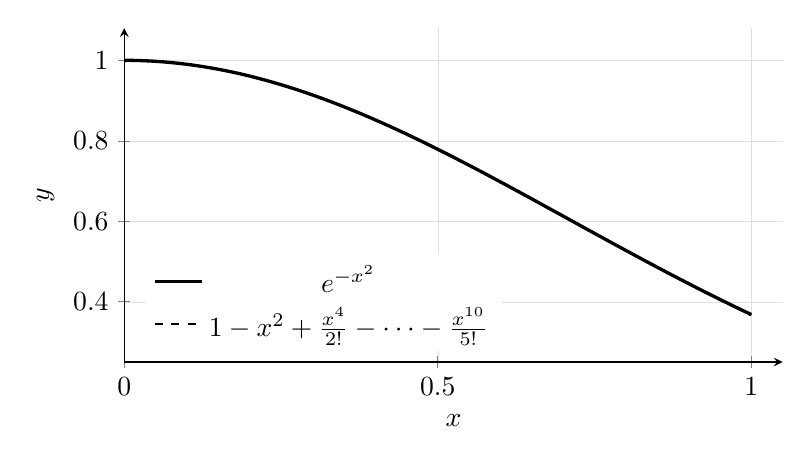
\begin{tikzpicture}
\begin{axis}[
    width=0.82\textwidth,
    height=0.48\textwidth,
    xmin=0, xmax=1.05,
    ymin=0.25, ymax=1.08,
    axis lines=left,
    xlabel={\(x\)},
    ylabel={\(y\)},
    xtick={0,0.5,1},
    ytick={0.4,0.6,0.8,1},
    grid=both,
    grid style={line width=.1pt, draw=gray!25},
    legend style={draw=none, at={(0.03,0.03)}, anchor=south west}
]
\addplot[very thick, domain=0:1, samples=200] {exp(-x^2)};
\addlegendentry{\(e^{-x^2}\)}

\addplot[thick, dashed, domain=0:1, samples=200] {1-x^2+x^4/2-x^6/6+x^8/24-x^10/120};
\addlegendentry{\(1-x^2+\frac{x^4}{2!}-\cdots-\frac{x^{10}}{5!}\)}
\end{axis}
\end{tikzpicture}
\caption{On \([0,1]\), a Taylor polynomial gives a close approximation to \(e^{-x^2}\), and integrating the polynomial gives an approximation to the area.}
\label{fig:gaussian-taylor-approx}
\end{figure}

This example shows a new use of series.  A function may have no elementary
antiderivative, but its Taylor series may integrate term by term into a useful numerical
answer.

\paragraph{Another short example.}
Approximate

\[
\int_0^{0.2}\frac{\sin x}{x}\,dx.
\]

The integrand is not defined by the formula at \(x=0\), but the limit exists.  Since

\[
\sin x=x-\frac{x^3}{3!}+\frac{x^5}{5!}-\cdots,
\]

we have, for \(x\neq0\),

\[
\frac{\sin x}{x}
=
1-\frac{x^2}{3!}+\frac{x^4}{5!}-\cdots.
\]

The limiting value at \(x=0\) is \(1\), so this series gives the continuous extension.

Integrate:

\[
\int_0^{0.2}\frac{\sin x}{x}\,dx
=
\int_0^{0.2}
\left(
1-\frac{x^2}{3!}+\frac{x^4}{5!}-\cdots
\right)dx.
\]

Using the first two terms,

\[
\int_0^{0.2}\frac{\sin x}{x}\,dx
\approx
0.2-\frac{(0.2)^3}{3\cdot 3!}.
\]

So

\[
\int_0^{0.2}\frac{\sin x}{x}\,dx
\approx
0.2-\frac{0.008}{18}
=
0.199555\ldots.
\]

The next term has size

\[
\frac{(0.2)^5}{5\cdot 5!}
=
\frac{0.00032}{600}
<0.000001.
\]

Thus the approximation is accurate to within \(0.000001\).

\subsection{Solving differential equations by series}
\label{subsec:solving-differential-equations-series}

A differential equation gives a law for an unknown function.  Sometimes the solution is
one of the familiar functions.  Sometimes it is not.

Power series give a way to build a solution from its coefficients.

The idea is to assume

\[
y=a_0+a_1x+a_2x^2+a_3x^3+\cdots,
\]

substitute into the differential equation, and match coefficients.

\paragraph{Example: the sine function from a differential equation.}
Solve

\[
y''+y=0,
\qquad
y(0)=0,
\qquad
y'(0)=1
\]

by a power series.

Assume

\[
y=\sum_{n=0}^{\infty}a_nx^n.
\]

Then

\[
y'=\sum_{n=1}^{\infty}n a_n x^{n-1},
\]

and

\[
y''=\sum_{n=2}^{\infty}n(n-1)a_nx^{n-2}.
\]

Rewrite \(y''\) so that the power is \(x^n\):

\[
y''=
\sum_{n=0}^{\infty}
(n+2)(n+1)a_{n+2}x^n.
\]

The equation \(y''+y=0\) becomes

\[
\sum_{n=0}^{\infty}
\bigl((n+2)(n+1)a_{n+2}+a_n\bigr)x^n=0.
\]

For this power series to be zero for all \(x\) near \(0\), each coefficient must be zero:

\[
(n+2)(n+1)a_{n+2}+a_n=0.
\]

Thus

\[
\boxed{
a_{n+2}=-\frac{a_n}{(n+2)(n+1)}.
}
\]

The initial conditions give

\[
y(0)=a_0=0,
\]

and

\[
y'(0)=a_1=1.
\]

Now use the recurrence.

Since \(a_0=0\),

\[
a_2=-\frac{a_0}{2\cdot1}=0.
\]

Since \(a_1=1\),

\[
a_3=-\frac{a_1}{3\cdot2}=-\frac1{3!}.
\]

Then

\[
a_4=0,
\]

and

\[
a_5=-\frac{a_3}{5\cdot4}
=
\frac1{5!}.
\]

Continuing,

\[
a_7=-\frac1{7!},
\qquad
a_9=\frac1{9!},
\qquad\ldots.
\]

So

\[
y=x-\frac{x^3}{3!}+\frac{x^5}{5!}-\frac{x^7}{7!}+\cdots.
\]

Therefore

\[
\boxed{
y=\sin x.
}
\]

The sine function is not just a triangle ratio.  It is also the solution of the differential
equation

\[
y''+y=0
\]

with the initial conditions

\[
y(0)=0,
\qquad
y'(0)=1.
\]

That fact will become important when we discuss oscillation.

\paragraph{Example: a series solution that is not elementary.}
Consider

\[
y''=xy,
\qquad
y(0)=1,
\qquad
y'(0)=0.
\]

Again assume

\[
y=\sum_{n=0}^{\infty}a_nx^n.
\]

Then

\[
y''=
\sum_{n=0}^{\infty}
(n+2)(n+1)a_{n+2}x^n.
\]

Also,

\[
xy=x\sum_{n=0}^{\infty}a_nx^n
=
a_0x+a_1x^2+a_2x^3+\cdots.
\]

The coefficient of \(x^0\) on the right is \(0\), so

\[
2a_2=0,
\qquad
a_2=0.
\]

For \(n\ge1\), the coefficient of \(x^n\) on the right is \(a_{n-1}\).  Hence

\[
(n+2)(n+1)a_{n+2}=a_{n-1},
\qquad n\ge1.
\]

The initial conditions give

\[
a_0=1,
\qquad
a_1=0.
\]

Now compute the first few coefficients:

\[
a_2=0,
\]

\[
a_3=\frac{a_0}{3\cdot2}=\frac16,
\]

\[
a_4=\frac{a_1}{4\cdot3}=0,
\]

\[
a_5=\frac{a_2}{5\cdot4}=0,
\]

\[
a_6=\frac{a_3}{6\cdot5}=\frac1{180}.
\]

So the solution begins

\[
\boxed{
y=1+\frac{x^3}{6}+\frac{x^6}{180}+\cdots.
}
\]

This differential equation leads to functions beyond the usual elementary list.  The
series is not a trick for re-discovering old functions; it is a way to create new ones.

\subsection{Error bounds in applications}
\label{subsec:error-bounds-applications-taylor}

In applications, an approximation is judged by the error the situation can tolerate.

A navigation problem, a physics simulation, and a classroom estimate may all use the
same Taylor series, but they may require different numbers of terms.

\paragraph{Example: the small-angle approximation.}
For small angles, in radians,

\[
\sin \theta\approx \theta.
\]

Taylor's theorem explains the error.  Since

\[
\sin \theta
=
\theta-\frac{\theta^3}{3!}+\frac{\theta^5}{5!}-\cdots,
\]

the first omitted term after using \(\sin\theta\approx\theta\) is approximately

\[
\frac{\theta^3}{6}.
\]

More rigorously, Taylor's theorem gives

\[
\sin\theta
=
\theta+\frac{f'''(c)}{3!}\theta^3
\]

for some \(c\) between \(0\) and \(\theta\).  Since

\[
|f'''(c)|=|-\cos c|\le1,
\]

we have

\[
\boxed{
|\sin\theta-\theta|\le \frac{|\theta|^3}{6}.
}
\]

If

\[
|\theta|\le0.1,
\]

then

\[
|\sin\theta-\theta|
\le
\frac{0.1^3}{6}
=
0.000166\ldots.
\]

So for angles within \(0.1\) radian of \(0\), the approximation \(\sin\theta\approx\theta\)
has absolute error less than \(0.00017\).

For \(5^\circ\),

\[
\theta=\frac{5\pi}{180}=\frac{\pi}{36}
\]

radians, so

\[
|\sin\theta-\theta|
\le
\frac{(\pi/36)^3}{6}
<0.00012.
\]

The approximation is good because the angle is small in radians.

\paragraph{Choosing enough terms from a tolerance.}
Suppose we want to approximate

\[
\cos(0.4)
\]

with error less than

\[
0.00001.
\]

The cosine series is alternating:

\[
\cos x
=
1-\frac{x^2}{2!}+\frac{x^4}{4!}-\frac{x^6}{6!}+\cdots.
\]

If we use terms through \(x^4\), the first omitted term has size

\[
\frac{0.4^6}{6!}.
\]

Now

\[
0.4^6=0.004096
\qquad\text{and}\qquad
6!=720.
\]

So

\[
\frac{0.4^6}{6!}
=
\frac{0.004096}{720}
<0.000006.
\]

This is already less than \(0.00001\).  Therefore

\[
\cos(0.4)
\approx
1-\frac{0.4^2}{2!}+\frac{0.4^4}{4!}
\]

meets the required tolerance.

Compute:

\[
1-\frac{0.16}{2}+\frac{0.0256}{24}
=
1-0.08+0.001066\ldots
=
0.921066\ldots.
\]

Thus

\[
\boxed{
\cos(0.4)\approx0.921067
}
\]

with error less than \(0.00001\).

\begin{quote}
\textbf{Practical Taylor workflow.}

\begin{enumerate}
\item Choose a center close to the input.

\item Write the Taylor series.

\item Use enough terms so that the remainder is below the desired tolerance.

\item State the approximation and the error bound together.
\end{enumerate}
\end{quote}

Taylor series turn functions into algorithms.  But the algorithms work because their
errors can be bounded.  The next section explains, in a preview form, why power series
allow such safe term-by-term work inside their radius of convergence.

\section{Uniform convergence preview}
\label{sec:uniform-convergence-preview}

Power series have been unusually obedient.  Inside their radius of convergence, we have
added them, multiplied them, differentiated them, integrated them, and used them to
represent functions.

This is not how arbitrary infinite sums of functions behave.

The missing idea is not another formula.  It is a stronger kind of convergence.

Ordinary convergence can happen separately at each point.  Uniform convergence means
the approximation is good on a whole interval at once.

\[
\boxed{
\text{Uniform convergence is convergence with one error bound for all points in a set.}
}
\]

This section is a preview.  A later analysis course will make these ideas fully systematic.
Here we use them to explain why power series are trustworthy inside their radius.

\subsection{Pointwise convergence of functions}
\label{subsec:pointwise-convergence-functions}

A sequence of numbers is a list:

\[
a_1,\ a_2,\ a_3,\ldots.
\]

A sequence of functions is a list of functions:

\[
f_1,\ f_2,\ f_3,\ldots.
\]

For example, on the interval \([0,1]\), define

\[
f_n(x)=x^n.
\]

Then

\[
f_1(x)=x,\qquad
f_2(x)=x^2,\qquad
f_3(x)=x^3,\qquad \ldots.
\]

For a fixed number \(x\) with

\[
0\le x<1,
\]

we have

\[
x^n\to0.
\]

But at \(x=1\),

\[
1^n=1
\]

for every \(n\).  So the limiting function is

\[
f(x)=
\begin{cases}
0, & 0\le x<1,\\
1, & x=1.
\end{cases}
\]

This means that \(f_n(x)=x^n\) converges to \(f(x)\) point by point.

\begin{quote}
\textbf{Pointwise convergence.}
A sequence of functions \(f_n\) converges \emph{pointwise} to a function \(f\) on a set
\(I\) if, for each fixed \(x\in I\),

\[
\lim_{n\to\infty}f_n(x)=f(x).
\]
\end{quote}

The words ``for each fixed \(x\)'' are important.  Pointwise convergence lets the speed
of convergence depend on the point.

Near \(x=0\), the powers \(x^n\) shrink quickly.  Near \(x=1\), they shrink slowly.

\begin{figure}[h]
\centering
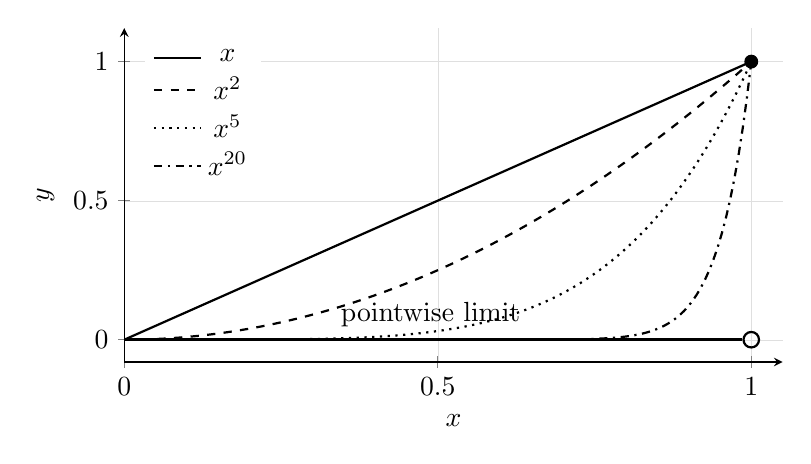
\begin{tikzpicture}
\begin{axis}[
    width=0.82\textwidth,
    height=0.48\textwidth,
    xmin=0, xmax=1.05,
    ymin=-0.08, ymax=1.12,
    axis lines=left,
    xlabel={\(x\)},
    ylabel={\(y\)},
    xtick={0,0.5,1},
    ytick={0,0.5,1},
    grid=both,
    grid style={line width=.1pt, draw=gray!25},
    legend style={draw=none, at={(0.03,0.97)}, anchor=north west}
]
\addplot[thick, domain=0:1, samples=150] {x};
\addlegendentry{\(x\)}

\addplot[thick, dashed, domain=0:1, samples=150] {x^2};
\addlegendentry{\(x^2\)}

\addplot[thick, dotted, domain=0:1, samples=150] {x^5};
\addlegendentry{\(x^5\)}

\addplot[thick, dashdotted, domain=0:1, samples=150] {x^20};
\addlegendentry{\(x^{20}\)}

\addplot[very thick, domain=0:0.985, samples=2] {0};
\addplot[only marks, mark=o, mark size=2.8pt, thick] coordinates {(1,0)};
\addplot[only marks, mark=*, mark size=2.3pt] coordinates {(1,1)};
\node[anchor=west] at (axis cs:0.33,0.09) {pointwise limit};
\end{axis}
\end{tikzpicture}
\caption{The functions \(x^n\) converge pointwise on \([0,1]\), but the convergence is slow near \(x=1\).}
\label{fig:pointwise-xn}
\end{figure}

A surprising thing happened: every \(f_n(x)=x^n\) is continuous, but the pointwise
limit is not continuous.  The limit jumps at \(x=1\).

This is our first warning that pointwise convergence is too weak to preserve all the good
behavior of the approximating functions.

\subsection{Uniform convergence as one error bound for all points}
\label{subsec:uniform-convergence-one-error-bound}

Uniform convergence strengthens pointwise convergence by requiring one \(N\) that
works for every point in the set.

\begin{quote}
\textbf{Uniform convergence.}
A sequence of functions \(f_n\) converges \emph{uniformly} to \(f\) on a set \(I\) if, for
every \(\varepsilon>0\), there is an integer \(N\) such that

\[
|f_n(x)-f(x)|<\varepsilon
\]

for every \(x\in I\) whenever \(n\ge N\).
\end{quote}

Compare the two ideas.

\begin{center}
\renewcommand{\arraystretch}{1.4}
\begin{tabular}{c|c}
\textbf{pointwise convergence} & \textbf{uniform convergence} \\ \hline
For each \(x\), find an \(N\). & Find one \(N\) that works for all \(x\). \\
The speed may depend on \(x\). & The error is controlled on the whole set. \\
Good at individual points. & Good on an interval all at once.
\end{tabular}
\end{center}

\paragraph{Example: uniform convergence on a smaller interval.}
The functions

\[
f_n(x)=x^n
\]

do not converge uniformly to \(0\) on \([0,1)\).  But they do converge uniformly to \(0\)
on any interval

\[
[0,r]
\]

where

\[
0<r<1.
\]

Indeed, if \(0\le x\le r\), then

\[
0\le x^n\le r^n.
\]

Since

\[
r^n\to0,
\]

we can make \(r^n\) smaller than any chosen \(\varepsilon\).  Then

\[
|x^n-0|<\varepsilon
\]

for every \(x\in[0,r]\) at once.

The endpoint \(1\) was the problem.  Staying a fixed distance away from it gives a
uniform error bound.

\paragraph{Why \(x^n\) is not uniform on \([0,1)\).}
For each fixed \(x<1\),

\[
x^n\to0.
\]

But no single \(N\) controls all \(x<1\).  To see why, choose

\[
x_n=\left(\frac34\right)^{1/n}.
\]

Then

\[
0<x_n<1,
\]

but

\[
x_n^n=\frac34.
\]

So no matter how large \(n\) is, there is a point \(x_n\) close enough to \(1\) where the
error is still

\[
\frac34.
\]

The convergence is pointwise, but not uniform.

\paragraph{Example: geometric series with a uniform error bound.}
Let

\[
S_N(x)=1+x+x^2+\cdots+x^N.
\]

For \(|x|<1\),

\[
S_N(x)\to \frac1{1-x}.
\]

The exact remainder is

\[
\frac1{1-x}-S_N(x)
=
\frac{x^{N+1}}{1-x}.
\]

Now choose a number \(r\) with

\[
0<r<1.
\]

On the closed interval

\[
[-r,r],
\]

we have

\[
|x|\le r
\]

and

\[
|1-x|\ge 1-r.
\]

Therefore

\[
\left|
\frac1{1-x}-S_N(x)
\right|
\le
\frac{r^{N+1}}{1-r}.
\]

The right side does not depend on \(x\).  Since

\[
\frac{r^{N+1}}{1-r}\to0,
\]

the convergence is uniform on \([-r,r]\).

This is the key pattern for power series:

\[
\boxed{
\text{inside the radius, leave a safety margin; then one error bound controls the interval.}
}
\]

\subsection{Interchanging limits and integrals}
\label{subsec:interchanging-limits-integrals}

Uniform convergence matters because it allows us to pass limits through integrals.

\begin{quote}
\textbf{Uniform convergence and integrals.}
Suppose \(f_n\) are continuous on \([a,b]\), and

\[
f_n\to f
\]

uniformly on \([a,b]\).  Then

\[
\boxed{
\lim_{n\to\infty}\int_a^b f_n(x)\,dx
=
\int_a^b f(x)\,dx.
}
\]

Equivalently,

\[
\boxed{
\int_a^b \left(\lim_{n\to\infty} f_n(x)\right)dx
=
\lim_{n\to\infty}\int_a^b f_n(x)\,dx.
}
\]
\end{quote}

Here is the reason.

If the convergence is uniform, then for a chosen error \(\varepsilon>0\), we can make

\[
|f_n(x)-f(x)|
<
\frac{\varepsilon}{b-a}
\]

for every \(x\in[a,b]\) once \(n\) is large enough.  Then

\[
\left|
\int_a^b f_n(x)\,dx-\int_a^b f(x)\,dx
\right|
=
\left|
\int_a^b \bigl(f_n(x)-f(x)\bigr)\,dx
\right|.
\]

By the triangle inequality for integrals,

\[
\left|
\int_a^b \bigl(f_n(x)-f(x)\bigr)\,dx
\right|
\le
\int_a^b |f_n(x)-f(x)|\,dx.
\]

So

\[
\int_a^b |f_n(x)-f(x)|\,dx
<
\int_a^b \frac{\varepsilon}{b-a}\,dx
=
\varepsilon.
\]

Thus the integrals converge to the integral of the limit.

Uniform convergence gives one error bound for the whole interval, so the accumulated
error is controlled.

\paragraph{Example: integrating the geometric series.}
For \(|t|<1\),

\[
\frac1{1-t}=1+t+t^2+t^3+\cdots.
\]

Fix an \(x\) with \(|x|<1\).  Choose \(r\) such that

\[
|x|<r<1.
\]

On the interval between \(0\) and \(x\), the geometric series converges uniformly,
because that interval lies inside \([-r,r]\).  Therefore we may integrate term by term:

\[
\int_0^x \frac1{1-t}\,dt
=
\int_0^x (1+t+t^2+t^3+\cdots)\,dt.
\]

The left side is

\[
-\ln(1-x).
\]

The right side is

\[
x+\frac{x^2}{2}+\frac{x^3}{3}+\frac{x^4}{4}+\cdots.
\]

Thus

\[
\boxed{
-\ln(1-x)
=
\sum_{n=1}^{\infty}\frac{x^n}{n},
\qquad |x|<1.
}
\]

Replacing \(x\) by \(-x\) gives the familiar series

\[
\ln(1+x)
=
x-\frac{x^2}{2}+\frac{x^3}{3}-\frac{x^4}{4}+\cdots.
\]

The term-by-term integration was not symbol pushing.  It was justified by uniform
control on a smaller closed interval inside the radius of convergence.

\paragraph{Why pointwise convergence is not enough.}
Pointwise convergence can fail to control area.

For example, on \([0,1]\), define a triangular spike \(g_n\) by

\[
g_n(x)=
\begin{cases}
n^2x, & 0\le x\le \frac1n,\\
2n-n^2x, & \frac1n<x\le \frac2n,\\
0, & \frac2n<x\le1.
\end{cases}
\]

Each \(g_n\) is a triangle with base

\[
\frac2n
\]

and height

\[
n.
\]

So its area is

\[
\frac12\cdot \frac2n\cdot n=1.
\]

For each fixed \(x>0\), eventually

\[
x>\frac2n,
\]

so

\[
g_n(x)=0.
\]

Also,

\[
g_n(0)=0.
\]

Thus

\[
g_n(x)\to0
\]

pointwise on \([0,1]\).  But

\[
\int_0^1 g_n(x)\,dx=1
\]

for every \(n\), while

\[
\int_0^1 0\,dx=0.
\]

So

\[
\lim_{n\to\infty}\int_0^1 g_n(x)\,dx
\neq
\int_0^1 \lim_{n\to\infty}g_n(x)\,dx.
\]

The spike gets narrower, but taller.  It disappears at each fixed point, yet it keeps area
\(1\).  Pointwise convergence did not control accumulated error.

\begin{quote}
\textbf{Moral.}
Pointwise convergence answers a point-by-point question.

Uniform convergence answers an interval-wide error question.

Integrals need interval-wide control.
\end{quote}

\subsection{Why power series are trustworthy inside their radius}
\label{subsec:why-power-series-trustworthy}

Power series are special because, inside their radius of convergence, they come with a
geometric safety margin.

Let

\[
F(x)=\sum_{n=0}^{\infty}c_n(x-a)^n
\]

have radius of convergence \(R>0\).  Choose a smaller radius \(r\) such that

\[
0<r<R.
\]

We will look only on the closed interval

\[
a-r\le x\le a+r.
\]

This interval stays safely inside the radius.

Now choose a number \(\rho\) such that

\[
r<\rho<R.
\]

Since \(\rho\) lies inside the radius of convergence,

\[
\sum_{n=0}^{\infty}|c_n|\rho^n
\]

converges.

For every \(x\) with

\[
|x-a|\le r,
\]

we have

\[
|c_n(x-a)^n|
\le
|c_n|r^n
\le
|c_n|\rho^n.
\]

The series

\[
\sum_{n=0}^{\infty}|c_n|\rho^n
\]

is a convergent numerical series independent of \(x\).  Therefore the power series is
controlled uniformly on

\[
[a-r,a+r].
\]

This is the uniform-convergence reason behind the safe operations.

\begin{quote}
\textbf{Power series inside their radius.}
A power series converges uniformly on every closed interval that stays strictly inside
its radius of convergence.

That is, if

\[
r<R,
\]

then

\[
\sum_{n=0}^{\infty}c_n(x-a)^n
\]

converges uniformly for

\[
|x-a|\le r.
\]
\end{quote}

The same safety margin also controls differentiated and integrated series.

For differentiation, the new terms are

\[
n c_n(x-a)^{n-1}.
\]

The extra factor \(n\) looks dangerous, but the geometric safety margin absorbs it.

Since

\[
\sum |c_n|\rho^n
\]

converges, the terms \(|c_n|\rho^n\) are bounded by some number \(M\).  For
\(|x-a|\le r\),

\[
n|c_n||x-a|^{n-1}
\le
\frac{M}{\rho}\, n\left(\frac{r}{\rho}\right)^{n-1}.
\]

Because

\[
0<\frac{r}{\rho}<1,
\]

the numerical series

\[
\sum_{n=1}^{\infty} n\left(\frac{r}{\rho}\right)^{n-1}
\]

converges.  So the differentiated series is also uniformly controlled on \([a-r,a+r]\).

This explains the theorem from Section \ref{subsec:differentiating-power-series}:

\[
\frac{d}{dx}\left(\sum_{n=0}^{\infty}c_n(x-a)^n\right)
=
\sum_{n=1}^{\infty}n c_n(x-a)^{n-1}
\]

inside the radius of convergence.

Integration is even gentler.  The integrated terms are

\[
c_n\frac{(x-a)^{n+1}}{n+1}.
\]

The factor \(1/(n+1)\) helps rather than hurts.  Uniform convergence allows

\[
\int \left(\sum_{n=0}^{\infty}c_n(x-a)^n\right)dx
=
C+\sum_{n=0}^{\infty}c_n\frac{(x-a)^{n+1}}{n+1}
\]

inside the radius.

\begin{quote}
\textbf{The safety-margin rule.}
Power series may be manipulated like polynomials on intervals that stay strictly inside
their radius of convergence.

At the endpoints, the safety margin disappears.  Endpoint behavior must be tested
separately.
\end{quote}

This is the hidden reason the earlier sections worked.  When we integrated

\[
1-x+x^2-x^3+\cdots
\]

to get

\[
\ln(1+x),
\]

we were working inside \(|x|<1\), where uniform control is available on every smaller
closed interval.

When we differentiated the geometric series to get

\[
\frac1{(1-x)^2}=1+2x+3x^2+4x^3+\cdots,
\]

we were again working inside the radius.

The endpoint behavior was never automatic.  It had to be checked separately.

Uniform convergence explains the good behavior of power series inside the radius.  The
next section shows what can go wrong when we forget the warnings: Taylor series may
have surprising endpoint behavior, term-by-term operations may fail for arbitrary
function series, and a Taylor series may even converge without converging to the function
that produced it.

\section{Warning examples}
\label{sec:warning-examples-taylor-series}

Uniform convergence explained why power series behave so well inside their radius.
That explanation should not make us careless.  Infinite processes are powerful because
they are controlled.  When the control is missing, familiar-looking operations can fail.

This section collects the warnings that belong at the end of the story.

\[
\boxed{
\text{A Taylor series is not automatically the function that produced it.}
}
\]

\[
\boxed{
\text{Endpoint behavior is not decided by the interior.}
}
\]

\[
\boxed{
\text{Term-by-term operations need hypotheses.}
}
\]

\subsection{A Taylor series can converge but not to the function}
\label{subsec:taylor-series-not-function}

The most surprising warning is this: all derivatives at one point may fail to determine
the function near that point.

Define

\[
f(x)=
\begin{cases}
e^{-1/x^2}, & x\neq0,\\
0, & x=0.
\end{cases}
\]

For \(x\neq0\), the function is positive.  For example,

\[
f(1)=e^{-1}>0.
\]

But near \(0\), the values are extremely small.  The factor \(e^{-1/x^2}\) goes to \(0\)
faster than any power of \(x\).

\begin{figure}[h]
\centering
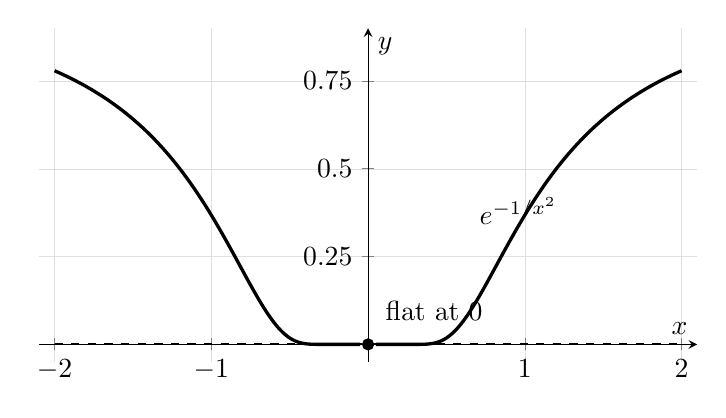
\begin{tikzpicture}
\begin{axis}[
    width=0.82\textwidth,
    height=0.48\textwidth,
    xmin=-2.1, xmax=2.1,
    ymin=-0.05, ymax=0.9,
    axis lines=middle,
    xlabel={\(x\)},
    ylabel={\(y\)},
    xtick={-2,-1,0,1,2},
    ytick={0,0.25,0.5,0.75},
    grid=both,
    grid style={line width=.1pt, draw=gray!25},
]
\addplot[very thick, domain=-2:-0.05, samples=200] {exp(-1/(x^2))};
\addplot[very thick, domain=0.05:2, samples=200] {exp(-1/(x^2))};
\addplot[only marks, mark=*] coordinates {(0,0)};
\addplot[thick, dashed, domain=-2:2, samples=2] {0};
\node[anchor=west] at (axis cs:0.65,0.38) {\(e^{-1/x^2}\)};
\node[anchor=south west] at (axis cs:0.05,0.04) {flat at \(0\)};
\end{axis}
\end{tikzpicture}
\caption{The function \(e^{-1/x^2}\), with \(f(0)=0\), is positive away from \(0\) but is infinitely flat at \(0\).}
\label{fig:flat-function}
\end{figure}

Let us compute the first derivative at \(0\).  By definition,

\[
f'(0)=\lim_{h\to0}\frac{f(h)-f(0)}{h}
=
\lim_{h\to0}\frac{e^{-1/h^2}}{h}.
\]

The numerator goes to \(0\) faster than the denominator goes to \(0\), so

\[
f'(0)=0.
\]

The same phenomenon happens for every higher derivative.  For \(x\neq0\), each
derivative has the form

\[
f^{(n)}(x)=P_n\left(\frac1x\right)e^{-1/x^2},
\]

where \(P_n\) is some polynomial.  The polynomial may grow as \(x\to0\), but the
exponential factor still wins.  Therefore

\[
f^{(n)}(0)=0
\]

for every \(n\ge0\).

So the Taylor series of \(f\) centered at \(0\) is

\[
\sum_{n=0}^{\infty}\frac{f^{(n)}(0)}{n!}x^n
=
0+0x+0x^2+0x^3+\cdots.
\]

Thus the Taylor series is the zero series:

\[
\boxed{
0.
}
\]

This series converges for every \(x\).  But it does not equal \(f(x)\) when \(x\neq0\),
because

\[
f(x)=e^{-1/x^2}>0.
\]

So we have found a function whose Taylor series converges everywhere but agrees with
the function only at the center.

\begin{quote}
\textbf{Moral.}
The Taylor series is built from derivative data at one point.  That data can be
insufficient.  To prove that a Taylor series equals a function, we need the remainder
to satisfy

\[
R_n(x)\to0.
\]
\end{quote}

This is why Taylor's theorem was not optional bookkeeping.  The remainder is the
bridge between the Taylor polynomials and the function.

\subsection{Endpoint behavior differs from interior behavior}
\label{subsec:endpoint-behavior-differs}

Inside the radius of convergence, power series behave predictably.  They converge
absolutely.  They can be differentiated and integrated term by term.

At the endpoints, that safety margin disappears.

Several power series have the same radius but different endpoint behavior:

\begin{center}
\renewcommand{\arraystretch}{1.45}
\begin{tabular}{c|c|c}
\textbf{series} & \textbf{radius} & \textbf{interval of convergence} \\ \hline
\(\displaystyle \sum_{n=0}^{\infty}x^n\) &
\(1\) &
\((-1,1)\) \\

\(\displaystyle \sum_{n=1}^{\infty}\frac{x^n}{n}\) &
\(1\) &
\([-1,1)\) \\

\(\displaystyle \sum_{n=1}^{\infty}(-1)^{n-1}\frac{x^n}{n}\) &
\(1\) &
\((-1,1]\) \\

\(\displaystyle \sum_{n=1}^{\infty}\frac{x^n}{n^2}\) &
\(1\) &
\([-1,1]\)
\end{tabular}
\end{center}

The radius only tells us what happens when

\[
|x|<1
\]

and when

\[
|x|>1.
\]

It does not decide what happens at

\[
x=-1
\qquad\text{or}\qquad
x=1.
\]

Those endpoints become ordinary numerical series, and ordinary series tests must be
used.

\paragraph{Differentiation can lose endpoints.}
Consider

\[
F(x)=\sum_{n=1}^{\infty}\frac{x^n}{n}.
\]

Its interval of convergence is

\[
[-1,1).
\]

Inside \((-1,1)\), differentiate term by term:

\[
F'(x)=\sum_{n=1}^{\infty}x^{n-1}.
\]

This derivative series is geometric:

\[
1+x+x^2+x^3+\cdots.
\]

Its interval of convergence is

\[
(-1,1).
\]

So the original series converged at \(x=-1\), but the differentiated series does not.

\paragraph{Integration can gain endpoints.}
Start with the geometric series:

\[
1+x+x^2+x^3+\cdots,
\qquad |x|<1.
\]

Integrate from \(0\) to \(x\):

\[
x+\frac{x^2}{2}+\frac{x^3}{3}+\frac{x^4}{4}+\cdots.
\]

The original geometric series diverges at both endpoints.  The integrated series
converges at \(x=-1\) by the Alternating Series Test, but diverges at \(x=1\) as the
harmonic series.

So the integrated series has interval

\[
[-1,1).
\]

The radius stayed the same.  The endpoint behavior changed.

\begin{quote}
\textbf{Endpoint rule.}
Differentiation and integration preserve the radius of convergence, but they do not
preserve endpoint behavior.

After any term-by-term operation, test endpoints again.
\end{quote}

\subsection{Termwise operations can fail for arbitrary function series}
\label{subsec:termwise-operations-fail}

Power series behave well inside their radius because they have geometric control.
Arbitrary infinite sums of functions may have no such control.

Here is a concrete failure for integration.

For \(n\ge2\), define a triangular spike on \([0,1]\):

\[
g_n(x)=
\begin{cases}
n^2x, & 0\le x\le \frac1n,\\[4pt]
2n-n^2x, & \frac1n<x\le \frac2n,\\[4pt]
0, & \frac2n<x\le1.
\end{cases}
\]

Each \(g_n\) is a triangle with base

\[
\frac2n
\]

and height

\[
n.
\]

Therefore

\[
\int_0^1 g_n(x)\,dx
=
\frac12\cdot \frac2n\cdot n
=
1.
\]

For each fixed \(x>0\), eventually \(x>\frac2n\), so

\[
g_n(x)=0.
\]

Also,

\[
g_n(0)=0.
\]

Thus

\[
g_n(x)\to0
\]

pointwise on \([0,1]\), even though every spike has area \(1\).

Now define

\[
h_n(x)=g_n(x)-g_{n+1}(x),
\qquad n\ge2.
\]

The series

\[
\sum_{n=2}^{\infty} h_n(x)
\]

telescopes.  Its \(N\)-th partial sum is

\[
S_N(x)=\sum_{n=2}^{N}h_n(x)
=
g_2(x)-g_{N+1}(x).
\]

Since \(g_{N+1}(x)\to0\) pointwise,

\[
S_N(x)\to g_2(x).
\]

Therefore

\[
\sum_{n=2}^{\infty}h_n(x)=g_2(x)
\]

pointwise.

Now compare the two ways of integrating.

First integrate the pointwise sum:

\[
\int_0^1 \left(\sum_{n=2}^{\infty}h_n(x)\right)dx
=
\int_0^1 g_2(x)\,dx
=
1.
\]

But each \(h_n\) has integral

\[
\int_0^1 h_n(x)\,dx
=
\int_0^1 g_n(x)\,dx-\int_0^1 g_{n+1}(x)\,dx
=
1-1
=
0.
\]

So

\[
\sum_{n=2}^{\infty}\int_0^1 h_n(x)\,dx
=
0.
\]

Thus

\[
\boxed{
\int_0^1 \left(\sum_{n=2}^{\infty}h_n(x)\right)dx
\neq
\sum_{n=2}^{\infty}\int_0^1 h_n(x)\,dx.
}
\]

The failure came from the moving spike.  The spike disappears at every fixed point, but
its area does not disappear.  Pointwise convergence did not control the accumulated
error.

\paragraph{Differentiation has its own warning.}
Even uniform convergence of functions is not enough to justify differentiating limits.

On \([-1,1]\), define

\[
F_n(x)=\sqrt{x^2+\frac1n}.
\]

Each \(F_n\) is differentiable.  Also,

\[
F_n(x)\to |x|
\]

uniformly on \([-1,1]\).  Indeed,

\[
0\le F_n(x)-|x|
\le \frac1{\sqrt n}.
\]

But the limit function

\[
|x|
\]

is not differentiable at \(0\).

So differentiating the approximating functions did not guarantee differentiability of the
limit.  To pass derivatives through a limit or an infinite sum, we need extra control,
usually control of the derivative series itself.

\begin{quote}
\textbf{Moral.}
Pointwise convergence is usually too weak for term-by-term operations.

Power series are special because they converge uniformly on every closed interval
strictly inside their radius of convergence.
\end{quote}

\subsection{A good local approximation can become bad far away}
\label{subsec:local-approximation-bad-far-away}

Taylor polynomials are local approximations.  They are built from derivative information
at one center.  A polynomial that is excellent near the center can be useless far away.

The geometric series gives the clearest example:

\[
\frac1{1-x}=1+x+x^2+x^3+\cdots,
\qquad |x|<1.
\]

The degree \(N\) partial sum is

\[
S_N(x)=1+x+x^2+\cdots+x^N.
\]

For \(|x|<1\),

\[
\frac1{1-x}-S_N(x)
=
\frac{x^{N+1}}{1-x}.
\]

At \(x=\frac12\),

\[
\left|
\frac1{1-\frac12}-S_N\left(\frac12\right)
\right|
=
\frac{(1/2)^{N+1}}{1/2}
=
\frac1{2^N}.
\]

So the approximation becomes excellent quickly.

But at \(x=2\), the function is perfectly defined:

\[
\frac1{1-2}=-1.
\]

The partial sums are

\[
S_N(2)=1+2+2^2+\cdots+2^N=2^{N+1}-1.
\]

These values grow without bound.  They do not approach \(-1\).

The problem is not that \(1/(1-x)\) is undefined at \(2\).  It is defined there.  The
problem is that the power series centered at \(0\) has radius \(1\).  The singularity at
\(x=1\) blocks the series before it can reach \(x=2\).

\begin{figure}[h]
\centering
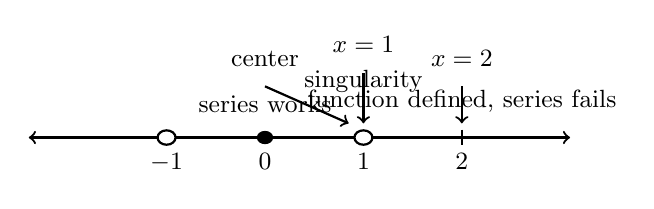
\begin{tikzpicture}[xscale=1.25, every node/.style={font=\small}]
  \draw[<->, thick] (-2.4,0) -- (3.1,0);

  \draw[very thick] (-1,0) -- (1,0);
  \draw[fill=white, thick] (-1,0) circle (2.6pt);
  \draw[fill=white, thick] (1,0) circle (2.6pt);
  \draw[fill=black] (0,0) circle (2.2pt);

  \draw[thick] (2,0.1) -- (2,-0.1);
  \node[below] at (0,-0.08) {\(0\)};
  \node[below] at (-1,-0.08) {\(-1\)};
  \node[below] at (1,-0.08) {\(1\)};
  \node[below] at (2,-0.08) {\(2\)};

  \node[above] at (0,0.2) {series works};
  \node[above] at (1,0.45) {singularity};
  \node[above] at (2,0.2) {function defined, series fails};

  \draw[->, thick] (0,0.65) -- (0.85,0.18);
  \node[above] at (0,0.78) {center};

  \draw[->, thick] (1,0.82) -- (1,0.18);
  \node[above] at (1,0.95) {\(x=1\)};

  \draw[->, thick] (2,0.65) -- (2,0.18);
  \node[above] at (2,0.78) {\(x=2\)};
\end{tikzpicture}
\caption{The Maclaurin series for \(\frac1{1-x}\) has radius \(1\).  It cannot pass the singularity at \(x=1\), even though the function is defined again at \(x=2\).}
\label{fig:local-series-radius-block}
\end{figure}

\begin{quote}
\textbf{Local approximation warning.}
A Taylor polynomial may be excellent near its center and poor far away.

A Taylor series may represent a function only on part of the function's domain.
\end{quote}

These warnings complete the chapter's main lesson.  Infinite polynomials are useful
because they come with a domain, a remainder, and a convergence story.  Without those
three pieces, the formulas are only formal patterns.

\section{Chapter review and projects}
\label{sec:chapter-review-power-taylor}

Chapter 16 started with infinite polynomials and ended with a warning about their
limits.  The main thread was approximation with control.

A power series is a function-building machine.  A Taylor polynomial is a finite local
approximation.  A Taylor series is what happens when the degree grows without bound.
Taylor's theorem tells us when the finite approximations actually approach the function.

\subsection{Skills: power series and Taylor series}
\label{subsec:skills-power-series-taylor-series}

Here are the main skills of the chapter.

\begin{center}
\renewcommand{\arraystretch}{1.45}
\begin{tabular}{c|l|l}
\textbf{skill} & \textbf{question} & \textbf{main tool} \\ \hline
Power series convergence &
Where does the infinite polynomial make sense? &
Ratio Test, Root Test, endpoint tests \\

Power series algebra &
Can I rewrite a function using a known series? &
Geometric series, substitution, algebra \\

Term-by-term calculus &
Can I differentiate or integrate the series? &
Work inside the radius; test endpoints again \\

Taylor polynomials &
Which polynomial matches derivatives at the center? &
\(\displaystyle T_n(x)=\sum_{k=0}^n\frac{f^{(k)}(a)}{k!}(x-a)^k\) \\

Taylor remainders &
How large can the error be? &
Lagrange remainder or alternating estimate \\

Taylor series &
Does the infinite Taylor series equal the function? &
Show \(R_n(x)\to0\)
\end{tabular}
\end{center}

The most common Maclaurin series are these:

\begin{center}
\renewcommand{\arraystretch}{1.7}
\begin{tabular}{c|c|c}
\textbf{function} & \textbf{Maclaurin series} & \textbf{where valid} \\ \hline
\(\displaystyle \frac1{1-x}\) &
\(\displaystyle \sum_{n=0}^{\infty}x^n\) &
\(|x|<1\) \\

\(e^x\) &
\(\displaystyle \sum_{n=0}^{\infty}\frac{x^n}{n!}\) &
all \(x\) \\

\(\sin x\) &
\(\displaystyle \sum_{n=0}^{\infty}(-1)^n\frac{x^{2n+1}}{(2n+1)!}\) &
all \(x\) \\

\(\cos x\) &
\(\displaystyle \sum_{n=0}^{\infty}(-1)^n\frac{x^{2n}}{(2n)!}\) &
all \(x\) \\

\(\ln(1+x)\) &
\(\displaystyle \sum_{n=1}^{\infty}(-1)^{n-1}\frac{x^n}{n}\) &
\(-1<x\le1\) \\

\(\arctan x\) &
\(\displaystyle \sum_{n=0}^{\infty}(-1)^n\frac{x^{2n+1}}{2n+1}\) &
\(-1\le x\le1\) \\

\((1+x)^p\) &
\(\displaystyle \sum_{n=0}^{\infty}\binom{p}{n}x^n\) &
\(|x|<1\), with endpoints tested separately
\end{tabular}
\end{center}

\begin{quote}
\textbf{Three questions to ask every time.}

When using a power series or Taylor series, ask:

\begin{enumerate}
\item What is the center?

\item Where does the series converge?

\item If it is a Taylor series, why does it equal the function?
\end{enumerate}
\end{quote}

\paragraph{Review problems.}

\subparagraph{Concept checks.}
\begin{enumerate}
\item Explain the difference between a Taylor polynomial and a Taylor series.

\item Why does a power series always converge at its center?

\item Why must endpoints be tested separately after the radius of convergence is found?

\item Give an example of a power series whose radius is \(1\) but whose interval of
convergence is \([-1,1)\).

\item Explain why

\[
\lim_{n\to\infty}T_n(x)=f(x)
\]

does not follow only from the fact that \(T_n\) is the \(n\)-th Taylor polynomial of \(f\).

\item What does the Lagrange remainder tell us that the Taylor polynomial alone does not?
\end{enumerate}

\subparagraph{Power series and intervals of convergence.}
Find the radius and interval of convergence.

\begin{enumerate}
\setcounter{enumi}{6}

\item
\[
\sum_{n=1}^{\infty} \frac{n(x-3)^n}{5^n}.
\]

\item
\[
\sum_{n=1}^{\infty}\frac{(x+2)^n}{n4^n}.
\]

\item
\[
\sum_{n=0}^{\infty}\frac{x^n}{n!}.
\]

\item
\[
\sum_{n=1}^{\infty}\frac{n!(x-1)^n}{n^n}.
\]

\item
\[
\sum_{n=1}^{\infty}\frac{(-1)^n(x+1)^n}{\sqrt n}.
\]
\end{enumerate}

\subparagraph{Represent functions by power series.}
Find a power series centered at \(0\), and state where it is valid.

\begin{enumerate}
\setcounter{enumi}{11}

\item
\[
\frac1{4+x}.
\]

\item
\[
\frac{x^2}{1+x^3}.
\]

\item
\[
\ln(1-x^2).
\]

\item
\[
\frac1{(1-2x)^2}.
\]

\item
\[
\int_0^x \frac{1}{1+t^4}\,dt.
\]
\end{enumerate}

\subparagraph{Taylor polynomials and Taylor series.}
\begin{enumerate}
\setcounter{enumi}{16}

\item Find the degree \(6\) Maclaurin polynomial for

\[
\cos(x^2).
\]

\item Find the degree \(5\) Maclaurin polynomial for

\[
e^{-2x}.
\]

\item Find the degree \(4\) Taylor polynomial for

\[
\ln x
\]

centered at \(x=1\).

\item Use the binomial series to find the first four nonzero terms of

\[
\frac1{\sqrt{1+x}}.
\]

\item Use Taylor series to evaluate

\[
\lim_{x\to0}\frac{e^x-1-x-\frac{x^2}{2}}{x^3}.
\]

\item Use Taylor series to evaluate

\[
\lim_{x\to0}\frac{\sin x-x}{x^3}.
\]

\item Use a Taylor series to approximate

\[
\int_0^{0.5} e^{-x^2}\,dx
\]

with an error less than \(0.0001\).

\item Find a power series solution, through terms of degree \(6\), for

\[
y'=xy,
\qquad
y(0)=1.
\]

\item Find a power series solution, through terms of degree \(7\), for

\[
y''+xy=0,
\qquad
y(0)=0,
\qquad
y'(0)=1.
\]
\end{enumerate}

\subparagraph{Error bounds.}
\begin{enumerate}
\setcounter{enumi}{25}

\item How many nonzero terms of the Maclaurin series for \(\sin x\) are enough to
approximate \(\sin(0.4)\) with error less than \(10^{-8}\)?

\item Use Taylor's theorem to approximate \(e^{0.1}\) with error less than \(10^{-6}\).

\item Use the alternating-series estimate to approximate \(\ln(1.2)\) with error less than
\(10^{-5}\).

\item Explain why the Maclaurin series for \(\ln(1+x)\) should not be used directly to
compute \(\ln 5\).

\item Give an example of a Taylor polynomial that is a good approximation near its center
but a poor approximation far away.  Explain what goes wrong.
\end{enumerate}

\subsection{Project: build a sine calculator with error control}
\label{subsec:project-sine-calculator}

A calculator does not know \(\sin x\) by magic.  Somewhere underneath, it uses identities,
approximations, and error control.

This project builds a simple version.

\paragraph{Goal.}
Write an algorithm that takes an angle \(x\), measured in radians, and a tolerance
\(\tau>0\), and returns a number \(S\) satisfying

\[
|\sin x-S|<\tau.
\]

Do not use a built-in sine function except to check your answers.

\paragraph{Step 1: reduce the angle.}
The Taylor series for sine works for every real \(x\), but it is fastest when \(|x|\) is small.

Use periodicity to replace \(x\) by an equivalent angle \(r\) with

\[
-\pi\le r\le \pi.
\]

One way is to choose an integer \(k\) near \(x/(2\pi)\) and set

\[
r=x-2\pi k.
\]

Then use symmetry to reduce further to

\[
-\frac{\pi}{2}\le r\le \frac{\pi}{2}.
\]

For example,

\[
\sin r=\sin(\pi-r)
\]

when

\[
\frac{\pi}{2}<r\le \pi,
\]

and

\[
\sin r=\sin(-\pi-r)
\]

when

\[
-\pi\le r<-\frac{\pi}{2}.
\]

After this reduction, \(\sin x=\sin r\), and the new input \(r\) has smaller absolute value.

\paragraph{Step 2: use the sine series.}
For \(|r|\le \pi/2\),

\[
\sin r
=
r-\frac{r^3}{3!}+\frac{r^5}{5!}-\frac{r^7}{7!}+\cdots.
\]

The terms alternate, and their absolute values decrease.  Therefore the error after
stopping is at most the first omitted term.

Instead of computing factorials each time, use the recurrence

\[
u_0=r,
\]

\[
u_{m+1}
=
-u_m\frac{r^2}{(2m+2)(2m+3)}.
\]

Then

\[
u_m=(-1)^m\frac{r^{2m+1}}{(2m+1)!}.
\]

The partial sum

\[
S_N=u_0+u_1+\cdots+u_N
\]

has error at most

\[
|u_{N+1}|.
\]

\paragraph{Step 3: stopping rule.}
Keep adding terms until the next term satisfies

\[
|u_{N+1}|<\tau.
\]

Then return

\[
S_N.
\]

The alternating-series estimate gives

\[
|\sin x-S_N|=|\sin r-S_N|<\tau.
\]

\paragraph{Deliverables.}
\begin{enumerate}
\item Write your algorithm in clear pseudocode or in a programming language.

\item Explain why the angle reduction does not change the sine value.

\item Prove the recurrence formula for \(u_{m+1}\).

\item Explain why the alternating-series error estimate applies after the angle has been
reduced to \([-\pi/2,\pi/2]\).

\item Test your calculator on

\[
x=0.1,\qquad x=1,\qquad x=10,\qquad x=100.
\]

For each input, record the reduced angle, the number of terms used, and the error when
compared with a built-in sine function.
\end{enumerate}

\paragraph{Reflection.}
Answer these questions after testing.

\begin{enumerate}
\item Why is angle reduction so helpful?

\item What happens if you try to compute \(\sin(100)\) using the Maclaurin series without
reducing the angle first?

\item Why is it dangerous to ask for an error tolerance much smaller than the precision of
the computer's arithmetic?
\end{enumerate}

\subsection{Project: compare Taylor approximations visually}
\label{subsec:project-compare-taylor-visually}

Taylor polynomials are easiest to understand when we see where they succeed and where
they fail.

\paragraph{Goal.}
Choose functions, plot their Taylor polynomials, and compare the approximation error
on different intervals.

\paragraph{Part A: choose functions.}
Choose at least three of the following:

\[
e^x,\qquad
\sin x,\qquad
\cos x,\qquad
\ln(1+x),\qquad
\frac1{1-x},\qquad
\sqrt{1+x}.
\]

For each function, use the Maclaurin polynomials of several degrees.

For example,

\[
T_1,\quad T_2,\quad T_4,\quad T_8.
\]

For \(\sin x\), use odd-degree Taylor polynomials:

\[
x,\qquad
x-\frac{x^3}{3!},\qquad
x-\frac{x^3}{3!}+\frac{x^5}{5!},\qquad \ldots.
\]

For \(\cos x\), use even-degree Taylor polynomials.

\paragraph{Part B: plot function and approximations.}
For each chosen function, make plots on at least two intervals:

\[
[-1,1]
\]

and a larger interval chosen to reveal failure or slower convergence.

Suggested larger intervals:

\[
[-4,4]\quad \text{for } e^x,\sin x,\cos x,
\]

\[
(-1,3]\quad \text{for } \ln(1+x),
\]

\[
[-2,2]\quad \text{for } \frac1{1-x},
\]

\[
(-1,3]\quad \text{for } \sqrt{1+x}.
\]

\paragraph{Part C: plot the error.}
For each Taylor polynomial, plot

\[
E_n(x)=|f(x)-T_n(x)|.
\]

Also compute the largest error on a smaller interval, such as

\[
[-0.5,0.5]
\]

or

\[
[-1,1].
\]

Record your results in a table:

\begin{center}
\renewcommand{\arraystretch}{1.35}
\begin{tabular}{c|c|c|c}
\textbf{function} & \textbf{degree} & \textbf{interval} & \textbf{largest observed error} \\ \hline
 & & & \\
 & & & \\
 & & &
\end{tabular}
\end{center}

\paragraph{Part D: explain what you see.}
Write a short report answering these questions.

\begin{enumerate}
\item Which functions are approximated well on the largest interval you tried?

\item Which functions show a clear boundary where the Taylor series stops working?

\item How does the radius of convergence appear in the graph?

\item How does increasing the degree change the approximation near the center?

\item How does increasing the degree change the approximation far from the center?

\item For \(\sin x\) and \(\cos x\), what symmetry do the Taylor polynomials preserve?
\end{enumerate}

\paragraph{Optional extension: the flat function.}
Plot

\[
f(x)=
\begin{cases}
e^{-1/x^2}, & x\neq0,\\
0, & x=0.
\end{cases}
\]

Compare it with its Taylor series centered at \(0\).  Explain why every Taylor polynomial
is the zero polynomial, even though the function is not zero away from \(0\).

\subsection{Hook: the series for sine and cosine hide a rotating vector}
\label{subsec:hook-sine-cosine-rotating-vector}

The chapter began with a promise from the end of the previous chapter:

\[
e^{i\theta}=\cos\theta+i\sin\theta.
\]

Now the formula no longer looks impossible.  We have the three series that will create it:

\[
e^x
=
1+x+\frac{x^2}{2!}+\frac{x^3}{3!}
+\frac{x^4}{4!}+\cdots,
\]

\[
\cos \theta
=
1-\frac{\theta^2}{2!}+\frac{\theta^4}{4!}
-\frac{\theta^6}{6!}+\cdots,
\]

\[
\sin \theta
=
\theta-\frac{\theta^3}{3!}+\frac{\theta^5}{5!}
-\frac{\theta^7}{7!}+\cdots.
\]

There is one new symbol we have not yet given a geometric home:

\[
i.
\]

It satisfies

\[
i^2=-1.
\]

If we formally put \(x=i\theta\) into the exponential series, we get

\[
e^{i\theta}
=
1+i\theta+\frac{(i\theta)^2}{2!}
+\frac{(i\theta)^3}{3!}
+\frac{(i\theta)^4}{4!}
+\cdots.
\]

Since

\[
i^2=-1,\qquad i^3=-i,\qquad i^4=1,
\]

the terms separate into two parts:

\[
e^{i\theta}
=
\left(
1-\frac{\theta^2}{2!}
+\frac{\theta^4}{4!}
-\cdots
\right)
+
i\left(
\theta-\frac{\theta^3}{3!}
+\frac{\theta^5}{5!}
-\cdots
\right).
\]

The first parentheses are \(\cos\theta\).  The second parentheses are \(\sin\theta\).
So the series suggest

\[
\boxed{
e^{i\theta}=\cos\theta+i\sin\theta.
}
\]

\begin{figure}[h]
\centering
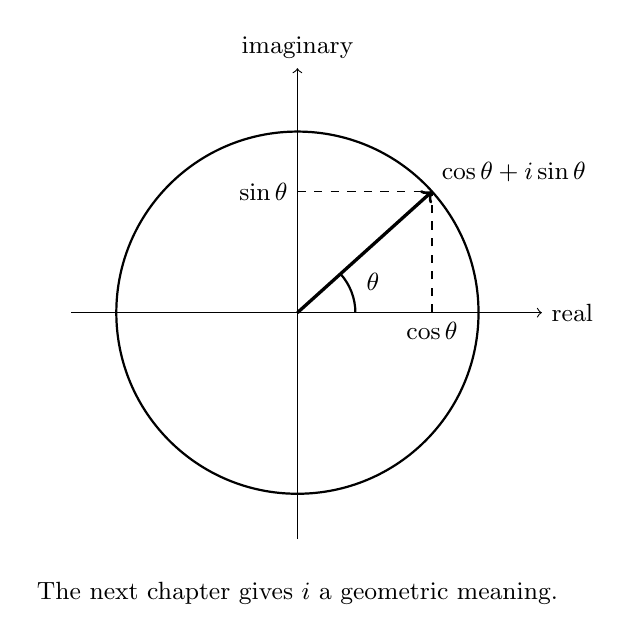
\begin{tikzpicture}[scale=2.3, every node/.style={font=\small}]
  \draw[->] (-1.25,0) -- (1.35,0) node[right] {real};
  \draw[->] (0,-1.25) -- (0,1.35) node[above] {imaginary};

  \draw[thick] (0,0) circle (1);

  \def\ang{42}
  \draw[very thick,->] (0,0) -- ({cos(\ang)},{sin(\ang)});
  \draw[thick] (0.32,0) arc (0:\ang:0.32);
  \node at ({0.45*cos(22)},{0.45*sin(22)}) {\(\theta\)};

  \draw[dashed] ({cos(\ang)},0) -- ({cos(\ang)},{sin(\ang)});
  \draw[dashed] (0,{sin(\ang)}) -- ({cos(\ang)},{sin(\ang)});

  \node[below] at ({cos(\ang)},0) {\(\cos\theta\)};
  \node[left] at (0,{sin(\ang)}) {\(\sin\theta\)};
  \node[above right] at ({cos(\ang)},{sin(\ang)}) {\(\cos\theta+i\sin\theta\)};

  \node at (0,-1.55) {The next chapter gives \(i\) a geometric meaning.};
\end{tikzpicture}
\caption{The Taylor series hint that \(e^{i\theta}\) traces the unit circle.}
\label{fig:euler-formula-hook}
\end{figure}

This is the doorway to the next chapter.  Complex numbers will turn \(i\) from a symbol
into a direction, and the exponential function will become a language for rotation.